\documentclass{article}
\usepackage{listings}
\usepackage{amsmath, amsthm, amssymb, amsfonts}
\usepackage{xcolor}
\usepackage{listings}
\usepackage{thmtools}
\usepackage{graphicx}
\usepackage{setspace}
\usepackage{geometry}
\usepackage{float}
\usepackage{hyperref}
\usepackage[utf8]{inputenc}
\usepackage[english]{babel}
\usepackage{framed}
\usepackage[dvipsnames]{xcolor}
\usepackage{xcolor}
\usepackage{tabularray}



\newcommand{\HRule}[1]{\rule{\linewidth}{#1}}


\setstretch{1.2}
\geometry{
    textheight=9in,
    textwidth=5.5in,
    top=1in,
    headheight=12pt,
    headsep=25pt,
    footskip=30pt
}

% ------------------------------------------------------------------------------

\begin{document}
\lstdefinestyle{yaml}{
     basicstyle=\color{blue}\footnotesize,
     rulecolor=\color{black},
     string=[s]{'}{'},
     stringstyle=\color{blue},
     comment=[l]{:},
     commentstyle=\color{black},
     morecomment=[l]{-}
 }
% ------------------------------------------------------------------------------
% Cover Page and ToC
% ------------------------------------------------------------------------------
\definecolor{dkgreen}{rgb}{0,0.6,0}
\definecolor{gray}{rgb}{0.5,0.5,0.5}
\definecolor{mauve}{rgb}{0.58,0,0.82}
\lstset{language=SQL,
  basicstyle={\small\ttfamily},
  belowskip=3mm,
  breakatwhitespace=true,
  breaklines=true,
  classoffset=0,
  columns=flexible,
  commentstyle=\color{dkgreen},
  framexleftmargin=0.25em,
  frameshape={}{yy}{}{}, %To remove to vertical lines on left, set `frameshape={}{}{}{}`
  keywordstyle=\color{blue},
  numbers=none, %If you want line numbers, set `numbers=left`
  numberstyle=\tiny\color{gray},
  showstringspaces=false,
  stringstyle=\color{mauve},
  tabsize=3,
  xleftmargin =1em
}
\title{ \normalsize \textsc{}
		\\ [2.0cm]
		\HRule{1.5pt} \\
		\LARGE \textbf{\uppercase{Documento di Note}
		\HRule{2.0pt} \\ [0.6cm] \LARGE{In questo documento vengono riportati i concetti affrontati durante lo stage presso Synclab S.r.L.} \vspace*{10\baselineskip}}
		}
\date{}
\author{\textbf{Author} \\ 
		Marco Brugin \\
		Synclab S.r.L. \\
		\today}

\maketitle
\newpage

\tableofcontents
\pagebreak
\listoffigures
\newpage

\section{Streaming ad eventi}
È una pratica di acquisizione dei dati in tempo reale da fonti di eventi come database, flussi di eventi; memorizzando tutto ciò per un recupero futuro di tali informazioni, reagendo a flussi di eventi in tempo reale. Inoltre garantisce un flusso  continuo di info corrette nel posto giusto e  al momento giusto.
\subsection{Utilizzi}
\begin{itemize}
    \item per transazioni
    \item per servizzi IOT di vario genere
    \item monitoraggio sanitario 
    \item ovunque ci sia la necessità di trattare grandi moli di dati efficientemente
\end{itemize}
\section{Apache \textbf{Kafka}}
\textbf{Kafka} è una piattaforma open source che combina 3 funzionalità in modo da poter soddisfare i casi d'uso sopra citati:
\begin{itemize}
    \item pubblica e sottoscrive flussi di eventi, importandoli ed 	esportandoli da altri sistemi;
    \item archivia tali flussi in modo affidabile e duraturo;	
    \item elabora flussi di eventi in real time o in modo retrospettivo.
\end{itemize}
\subsection{Utilizzo}
\textbf{Kafka} opera su una architettura distribuita. Può essere distribuito e utilizzato in vari modi tra cui virtual machine e container, on-promise, o servizi cloud.

\subsection{Funzionamento}
\textbf{Kafka} nasce come sistema distribuito che opera su nodi che comunicano tramite protocollo \textbf{TCP} ad alte prestazioni. Data la sua natura distribuita implementa capacità di fault tollerance con rimpiazzo dei nodi guasti. 
\textbf{Kafka} è costituito da due componenti essenziali: server e client.
\subsubsection{Server}
\textbf{Kafka} viene eseguito come un cluster di uno o più server. Alcuni fanno da \textbf{broker}: livello di archiviazione. Altri assolvono il compito di \textbf{\textbf{Kafka} Connect}: importano e esportano i dati sotto forma di  flussi di eventi che permette di interagire con altri sistemi esistenti.
\subsubsection{Client}
Consentono di scrivere applicazioni distribuite e microservizi che leggono, scrivono ed elaborano flussi di eventi in parallelo, su larga scala e con fault tollerance anche in caso di problemi di rete o guasti della macchina.
Esitono molti client per diversi linguaggi di programmazione.
\subsection{Garanzie di funzionamento}
In \textbf{Kafka} esistono produttori e consumatori che producono e sottoscrivono eventi. 
Gli uni sono sono indipendenti l'uno dall'altro, ciò permette di raggiungere alcune delle seguenti garanzie:
\begin{itemize}
    \item \textbf{Al massimo una volta}: i messaggipossono andare persi ma mai riconsegnati. Infatti si potrebbe verificare un guasto ad un singolo broker o un errore della rete nel momento dell'invio di un messaggio. Il messaggio stesso verrà recapitato una e una sola volta.
    \item \textbf{Almeno una volta}: i mesaggi non 		vengono mai persi ma possono essere 		riconsegnati;
    \item \textbf{Una solo volta}: i messaggi non  		vanno persi e sono consegnati una 		sola volta; è la garanzia maggiormente desiderabile.
\end{itemize}
\subsection{Gestione degli eventi}
Gli eventi sono organizzati in topic o argomenti. Gli eventi possono essere letti da più consumatori. 
Un evento anche se consumato non viene eliminato, può essere impostato un timeout di mantenimento dell'evento.
I topic sono partizionati su più nodi. Tale partizionamento consente ai client di leggere e scrivere dati da/a molti broker. Quando un nuovo evento viene emesso questo si aggiunge all rispettiva partizione. Sarà \textbf{\textbf{Kafka}} a garantire che gli eventi vengano letti nell'ordine in cui sono stati scritti.
\subsection{Interfacce presentì}
\subsubsection{\textbf{Kafka} Producer}
L’interfaccia Producer permette alle applicazioni di inviare i flussi di dati ai broker di un cluster di Apache per categorizzarli e salvarli (nei topic già citati).
\subsubsection{\textbf{Kafka} Consumer}
L’interfaccia Consumer consente ai consumatori di Apache \textbf{Kafka} di  ricevere l’accesso ai dati, salvati nei topic di un cluster.
 \subsubsection{\textbf{Kafka} Connect}
    L’interfaccia Connect  consente di impostare produttori e consumatori riutilizzabili che collegano i topic di \textbf{Kafka} con le applicazioni o le banche dati esistenti.
\subsection{Replicas}
Con il termine di \textbf{Kafka Replication} significa disporre di più copie dei dati, distribuite su più server/broker.
Ciò aiuta a mantenere alti livelli di disponibilità in caso di guasto. \\Le repliche sono permesse  a livello di partizione. kafka ne designa una chimata leader mentre le altre  sono partizioni follower o \textbf{in-sync}. Il numero totale di repliche incluso il leader costituisce il fattore di replicazione.
Il leader è responsabile della ricezione e dell'invio dei dati, per quella partizione.
Per mantenere questi cluster e gli argomenti/partizioni all'interno, Kafka ha un servizio centralizzato chiamato \textbf{Zookeeper}.

\subsection{Retention}
Con \textbf{Retention} in \textbf{Kafka} si intende la possibilità di controllare la dimensione dei registri degli argomenti ed evitare di superare le dimensioni del disco esistente.\\La conservazione può essere configurata o controllata in base alla dimensione dei log o in base alla durata configurata.
Tale configurazione può essere impostata a grana fine o a grana grossa per ogni argomento o per tutti gli argomenti.\\
\subsubsection{Retention basata sul tempo}
Una volta raggiunto il tempo di conservazione configurato per il segmento, questo viene contrassegnato per l'eliminazione o la compattazione in base al criterio di pulizia configurato. Il periodo di conservazione predefinito per i segmenti è di 7 giorni.
In ordine di importanza i parametri configurabili per la    \textbf{Retention} basata sul tempo sono in ordine di importanza e valutazione:
\begin{enumerate}
    \item log.retention.ms;
    \item log.retention.minutes;
    \item log.retention.hours.
\end{enumerate}
Nel momento in cui un parametro di livello di priorità superiore non è impostato si segue ciò che indica quello di livello appena inferiore.
\subsubsection{Retention basata sulle dimensione}
In questo caso si va 
configurare la dimensione massima di una struttura di dati di registro per una partizione di argomento. Una volta che la dimensione del registro raggiunge questa dimensione, inizia a rimuovere i segmenti dalla sua fine.
\\
In ordine di importanza i parametri configurabili per la    \textbf{Retention} basata dimensione sono in ordine di importanza e valutazione:
\begin{enumerate}
    \item log.segment.bytes: la dimensione massima di un singolo file di registro;
    \item log.retention.check.interval.ms: la frequenza in millisecondi con cui la pulizia del registro verifica se un registro è idoneo per l'eliminazione;
    \item log.segment.delete.delay.ms: la quantità di tempo da attendere prima di eliminare un file dal file system.
\end{enumerate}
\subsection{Zookeeper}
\textbf{Zookeeper} è un prodotto open-source che si occupa della sincronizzazione tra i cluster distribuiti e ne gestisce le configurazioni, il controllo e la denominazione.\\
Il protocollo \textbf{Zookeeper Atomic Broadcast (ZAB)} è il cervello dell'intero sistema.\\
Ogni replica o nodo invia a intervalli regolari un messaggio \textit{ Keep-Alive} a Zookeeper, informando così \textbf{Zookeeper} che è vivo e funzionante. \\
Se ebtro un tempo prestabilito il messaggio non viene ricevuto si presume che il nodo sia morto e se era un leadere se ne elegge un altro.\\
\textbf{Zookeeper} permette di definire dei parametri che consentono di capire quando un nodo è guasto e quanto i nodi follower sono in ritardo rispetto al leader.\\
Il parametro zookeeper.session.timeout.ms millisecondi è impostato su 6000 per impostazione predefinita: indica che ,se il leader non riceve l'evento \textit{ Keep-Alive} entro quel periodo temporale, detiene che quel nodo sia morto.\\
Il parametro replica.lag.max.messages, decide la differenza consentita tra \textbf{Replica's Offset
}e \textbf{Leader's Offset}. Se questa differenza è maggiore di replica.lag.max.message-1, il nodo viene considerato in ritardo e viene rimosso dall'elenco dei nodi in sincronizzazione dal leader. \\
Tutti i nodi che sono attivi e sincronizzati formano l' \textbf{In-Sync Replica Set}(\textbf{ISR}).\\
Ora, se tutti i nodi in sincronizzazione hanno applicato un messaggio ai rispettivi log, questo messaggio viene considerato confermato e quindi inviato ai consumatori. In questo modo, \textbf{Kafka} garantisce che un messaggio di cui è stato eseguito il commit non andrà perso, purché sia presente almeno una replica attiva e sincronizzata, in ogni momento.\\
Un nodo non sincronizzato può ricongiungersi all'\textbf{ISR} se può risincronizzarsi completamente di nuovo, anche se ha perso alcuni dati a causa del suo arresto anomalo.
\subsection{Kraft}
\textbf{Apache Kafka Raft (KRaft)} è il protocollo di consenso introdotto per rimuovere la dipendenza di \textbf{Apache Kafka} da \textbf{ZooKeeper} per la gestione dei metadati. Ciò semplifica enormemente l'architettura di \textbf{Kafka} consolidando la responsabilità dei metadati all'interno di \textbf{Kafka} stesso, anziché suddividerla tra due diversi sistemi: \textbf{ZooKeeper e Kafka}.\\
\textbf{KRaft} utilizza un modello di archiviazione di origine evento che garantisce che le macchine a stati interni possano sempre essere ricreate accuratamente. Il registro eventi utilizzato per archiviare questo stato
 viene periodicamente abbreviato da istantanee per garantire che il registro non possa crescere all'infinito.\\ Gli altri nodi all'interno del quorum seguono il leader  rispondendo agli eventi che crea e memorizza nel suo registro. Pertanto, se un nodo si ferma a causa di un evento di partizionamento, ad esempio, può recuperare rapidamente eventuali eventi persi accedendo al registro quando si ricongiunge. \\
 La natura basata sugli eventi del protocollo KRaft significa che, a differenza del leader basato su ZooKeeper, il leader del quorum non ha bisogno di caricare lo stato da ZooKeeper prima che diventi attivo. Quando la leadership cambia, il nuovo leader attivo ha già tutti i record di metadati impegnati in memoria. Inoltre, lo stesso meccanismo guidato dagli eventi utilizzato nel protocollo KRaft viene utilizzato per tenere traccia dei metadati nel cluster. 
\subsection{Casi d'uso}
\subsubsection{Notifica dell'evento}
\textbf{Kafka} permette di trasmette semplicemente eventi per avvisare altri sistemi di un cambiamento nel suo dominio.
\subsubsection{Trasferimento di stato portato da eventi}
In questo utilizzo il destinatario dell'evento ottiene anche i dati di cui ha bisogno per eseguire azioni aggiuntive sui dati richiesti.
\subsubsection{Approvvigionamento di eventi}
In questo caso il sistema consente di descrivere ogni cambiamento di stato in un sistema come un evento, con ogni evento registrato in sequenza cronologica. Di conseguenza, il flusso di eventi stesso diventa la principale fonte di verità del sistema.
\subsection{Applicazioni}
\subsubsection{Messaggistica}
I broker di messaggi vengono utilizzati per disaccoppiare l'elaborazione del messaggio dal produttore dello stesso.
\textbf{Kafka} rispetto ai sistemi di messaggistica tradizionale ha una migliore velocità, partizionamento integrato e tolleranza agli errori.
L'utilizzo è basso, ma in ambiti in cui si richiede una bassa latenza, le garanzie fornite da \textbf{Kafka} sono alla pari dei tradizionali sistemi di messagistica, che lo rendono lo rendono una buona soluzione per applicazioni di elaborazione di messaggi su larga scala.

\subsubsection{Monitoraggio di siti web}
È il caso d'uso d'origine di \textbf{Kafka} , ha la caratteristica di generare un elevato volume di messaggi. Lo scopo era quello di ricostruire le attività degli utenti come insieme di eventi genrati dalle azioni dell'utente.
\subsubsection{Metrica}
Indica l'aggregazione di dati di monitoraggio provenienti da varie fonti per eseguire statistiche.
\subsubsection{Aggregazione di registri}
\textbf{Kafka} ha anche la capacità di estrarre i dati dai file di log fisici e fornisce una astrazione di tali sotto forma di flusso di messaggi. Ciò permette di garantire una più bassa latenza di elaborazione e supporto per più origini dati.
\subsubsection{Elaborazione del flusso}
È possibile andare a creare una  data-pipeline in cui i dati grezzi vengono consumati dagli argomenti di \textbf{Kafka}, aggregati, trasformati fino ad ottenere unn dato elaborato.
\subsubsection{Approvvigionamento di eventi}
È possibile utilizzare  di \textbf{Kafka} in aplicazioni cui cambiamenti di stato vengono registrati come sequenze di record in ordine temporale. \textbf{Kafka} permette il supporto per dati di registro memorizzati molto grandi tanto che lo rende un ottimo back-end di tali applicazioni. 
\subsubsection{Registro commit}
\textbf{Kafka} può fungere da sorta di log di commit esterno per un sistema distribuito. Il registro aiuta a replicare i dati tra i nodi e funge da meccanismo di risincronizzazione per consentire ai nodi non allineati di ripristinare i propri dati.

\subsection{Apache Kafka VS EDA}
L'emissione di un evento indica che qualcosa è accaduto e può essere visto come un agglomerato di dati atomico in grado di soddisfare l'evento stesso. 
\textbf{Kafka} è un sistema di streaming di eventi che gestisce un flusso continuo di eventi. Inoltre Kafka memorizza tali in modo duraturo per il successivo recupero, analisi o elaborazione in tempo reale e li inoltri a varie destinazioni secondo necessità.
\\
D'altra parte in una \textbf{EDA} (Event Driven Architecture) viene generati degli eventi che un agente acquisisce e risponde a tale evento.
per utilizzare \textbf{Kafka} in un sistema \textbf{EDA} la chiave è andare a sfruttare il disaccopiamento: invece di effetuare un polling continuo di verifica della presenza di nuovi dati, basterà ascoltare il verificarsi di un evento per agire. Inoltre grazie all'approcio sviluppato da \textbf{Kafka} un evento una volta soddisfatto non viene eliminato, ma conservato per un periodo ti tempo predeterminato, pertanto un evento potrà essere letto da più consumatori e potrà essere utilizzato per soddisfare una varietà di richieste.
\section{Even Driven Architecture}
L'\textbf{Even Driven Architecture} è un pattern archietteturale basato su eventi: degli agenti, che sono in grado di ricevere tali eventi, agiranno solo nel momento in cui questi ultimi si verificheranno. 
Una architettura basato su eventi fornisce una serie di altri vantaggi basati sul disaccopiamento tra il produttore e il consumatore dell'evento, i quali, nel momento dell'emissione di quest'ultimo non è necessario siano sincroni ma possono andare a sfruttare una comunicazione di tipo asincrona. 
\subsection{Casi d'uso}
\subsection{Integrazioni esterne}
In molti sistemi quando di verifica un evento è necessario interagire con un servizio esterno. Grazie ad una architettura ad eventi, ogni servizio sarà indipendente l'uno dall'altro, così che se un servizio riscontra problemi nella sua esecuzione gli altri non ne risenteranno, data la loro indipendenza. Inoltre anche l'aggiunta di nuovi servizi ha nessun impatto. 
\subsection{Flussi di lavoro}
L'archiettetura \textbf{EDA} può essere anche impiegata nell'orchestrazione di un flusso di lavoro; nel quale ogni servizio è responsabile di un part del flusso indipendentemente dagli altri. Il fattore chiave è andare ad eseguire il rispettivo servizio all'emissione di un determinato evento.
\subsection{Trasferimento di Stato}
La modifica di un dato è un altro caso d'uso in cui l'architettura \textbf{EDA} può essere utilizzato per segnalare in tempo reale il mutamento di un dato in una detrminata struttura dati.
\subsection{Accoppiamento temporale}
Inoltre grazie ad un' architettura \textbf{EDA} si va a rimuovere l'accopiamento temporale tra chi efettua una chiamata e chi va a risponde a quest'ultima.
\section{Middleware}
Con il termine di \textbf{Middleware} si va ad intendere un insieme di pacchetti software che molte applicazioni utilizzano per comunicare tra di loro. Il \textbf{Middleware} funge da ponte tra tecnologie differenti in modo da poterle totalmente integrare.\\
L'architettura sottostante ad un \textbf{Middleware} non è altro che una \textbf{data-pipeline} nella quale i dati passano da una applicazione in connessione all'altra. \\
La chiave di utilizzo di un \textbf{Middleware} è che fornisce disaccopiamento tra i vari stadi di una \textbf{data-pipeline}.
\section{Panoramica design pattern architetturali}
\subsection{Layered-Architecture}
È un modello architetturale basato su più livelli orrizontali, in cui ciascuno svolge un compito specifico e ha detrminata responsabilità. Sebbene il pattern in sè non indichi il numero di livelli da utilizzare, è usuale creare architetture con al più quattro livelli: presentazione, business, persistenza e database.
In tale archittetura ogni livello è del tutto separato dagli altri: le modifiche apportate ad un livello non generano cambiamenti agli altri, per questo si parla di livelli isolati.
La comunicazione tra i livelli avviene in dall'alto verso il basso e in generale attraverso livelli chiusi: il passaggio delle informazione tra due o più livelli deve attraversare tutti i livelli intermedi.

\subsection{Client-server}
Nel pattern architetturale client-server ci sono due componenti essenziali: il client, che richiede un servizio o una prestazione, e il server che la fornisce. Il client espone porte di richesta, mentre il server espone porte di servizio. In tale architettura vige un tipo di collegamento Request-Response.
Uno dei principali vantaggi di tale pattern architetturale il calcolo centralizzato dei dati.
\pagebreak
\subsection{Pipe-filter}
Il modello architetturale \textbf{Pipe-Fileter} è caraterrizzato da trasformazioni successive del flusso di dati.
\\
I dati dall'origine vengono inviati dall'origine verso le porte di input del primo filtro, dove viene eseguita la prima elaborazione, quindi il prodotto dell'elaborazione viene fornito dallì'output all'input del filtro successivo e così via.
\\
Il fattore importante in tale pattern architetturale è l'ordine con cui vengono eseguiti tali filtri.
\subsection{Broker}
Il \textbf{Broker} pattern architetturale che può essere utilizzzato per sistemi software disaccopiati e distribuiti che interagiscono tramite chiamate remote.
Il pattern è formato da tre agenti:
\begin{itemize}
    \item il client: che accede a funzionalità del server inviando le richieste al broker;
    \item il server che mette a disposizione del client i propri servizzi attraverso il broker;
    \item il broker: riceve le richieste dai client, le archivia e una volta trovato il server appropiato inoltra la richiesta e trasmette il risultato al client.
\end{itemize}
\section{Publisher-Subscriber}
Il pattern architetturale \textbf{Publisher-Subscriber} è un modello di progettazione software, utilizzato nei sistemi distribuiti, che impiegano una comunicazione asincrona tra i vari componenti.\\
Sebbene vada ad utilizare tecniche già preesistenti come la sottoscrizione e l'accodamento di messaggi, la  chiave di sucesso di tale pattern è il totale disoccopiamento delle componenti: i componenti non sono a conoscenza dell'identità e della presenza degli altri.\\
Il modello Pub-SUb è nato dalla necessità del rendere i sistemi ridimensionabili in modo dinamico.
\subsection{Architettura}
Il Pub-Sub fornisce un sistema di scambio di messaggi tra editori e sottoscrittori. Lo scambio tra questi ultimi non avviene in modo diretto tra gli agenti appena illustrati, ma viene utilizzato un intermediario che raggruppa i messaggi per argomento e fornisce disaccopiamento tra le componenti.
\subsection{Vantaggi}
\begin{itemize}
    \item \textbf{Debole accopiamento tra le componenti}: che rende il sistema più flessibile e modificabile dinamicamente;
    \item \textbf{Elevata scalabilità}: non esiste limite al numero di publisher e subscriber che possano comunicare;
    \item \textbf{Utilizzo della comunicazione ascincrona ad eventi}: non necessità della sicnrona degli attori coninvolti nella comunicazione;
    \item \textbf{Indipendente dal protocollo di comunicazione}: è integrabile con qualsiasi protocollo di comunicazione e stack tecnologico.
\end{itemize}
\section{Streaming Data pipelines}
Con il termine di 
\textbf{data-pipelines} si intende un software che consente il fluire automatico di dati da un punto ad un altro del sistema.
Di solito le origini sono molteplici e generano dati ad altissima velocità.
\\
L'architettura che sta dietro a una \textbf{data-pilenes} consente di consumare, elebaorare, archiviare dati in tempo reale, man mano che vengono generati.
Tutto ciò consente analisi e reazioni più veloci ad esigenze sorte.
\\
In generale nelle pipeline dati tradizionali estraggono, trasformano e caricano i dati prima che possano essere utilizzati.
Ma data la enorme mole di dati che le \textbf{Streaming Data pipelines} sono sottoposte, tutto ciò non è possibile.
\subsection{Architettura}
Infatti per elaborare dati in streaming provenienti da sistemi come \textbf{Kafka} è necssario creare due livelli per l'elaborazione dati: 
\begin{itemize}
    \item \textbf{Archiviazione}:
    questo livello consente la memorizzazione
    dei dati, permettendo letture e scritture a basso costo in termini computazionali mantenendo l'ordine di arrivo dei dati;
    \item \textbf{Lavorazione}: elabora e consuma i dati del livello di archiviazione andando a segnalare a quest'ultimo i dati non più necessari.
\end{itemize}
\subsection{Obiettivi}
\begin{itemize}
    \item \textbf{Scalabilità}: il volume dei dati può crescere notevolmente nel tempo quindi è necessario archiviare i dati in un \textbf{data warehouse};
    \item \textbf{Durata e consistenza}: è importante considerare che i dati letti potrebbero essere già modificati o obsoleti, quindi è fondamentale disporre di strumenti di monitoraggio del flusso dati nel tempo;
    \item \textbf{Ordinare}: l'archiettura deve essere in grado di individuare la sequenza dei dati nel flusso;
    \item 
    \textbf{Tolleranza ai guasti}: lo streaming dei dati non smettono mai di fluire da varie sorgenti e il sitema deve prevenire le interuuzioni di alcuni sorgentii;
    \item 
    \textbf{Latenza}: data l'enorme mole di dati prodotti, se questi ultimi non vengono gestiti in tempo reale perdono di rillevanza e diventano inutilizzabili.
\end{itemize}
\clearpage
\subsection{Alta affidabilità}
Il concetto di alta affidabilità è essenzialmente alla capacità di un sistema di funzionare continuamente senza guasti in un detrminato periodo di tempo.\\
Per garantire tali prestazioni in generale è necessario seguire i seguenti principi:
\begin{itemize}
    \item \textbf{Crossover affidabile}: creazione di ridondanza eseguendo l atto di passare dal componente X al componente Y senza perdere dati o influire sulle prestazioni;
    \item \textbf{Bilancio del carico}:
    tecnica attraverso  la quale si va a ridristribuire
    il carico di elaborazione da su tutte le risorse del sistema in modo tale che nessuna sia sovraccaricata;
    \item \textbf{Rillevazione e gestione automatica dei guasti}:
    i guasti devono essere visibili e i  sistemi devono disporre di un sistema deve essere provvisto di un sistema automatico in grado di gestirli autonomamente.
\end{itemize}
\section{Architetture distribuite}
Con il termine \textbf{distribuito} si va ad intendere un'architettura nella quale i componenti non si trovano su un'unica macchina ma possono cooperare attraverso una rete di comunicazione per raggiungere un detrminato obiettivo.
\\Le principali caraterristiche che si riscontrano su tale archietettura sono:
\begin{itemize}
    \item l'elaborazione non è limitata a una sola macchina;
    \item Il middleware è un'infrastruttura che supporta adeguatamente lo sviluppo e l'esecuzione di applicazioni distribuite, fornendo un buffer tra le applicazioni e la rete. Svolge il ruolo di intermediario del sistema e gestisce o supporta i diversi componenti di un sistema distribuito;
    \item le basi di un'architettura distribuita sono la  trasparenza, affidabilità e disponibilità.
\end{itemize}
\subsection{Confronto tra  architetture centralizzate e distribuite}
\begin{figure}[H]
    \centering
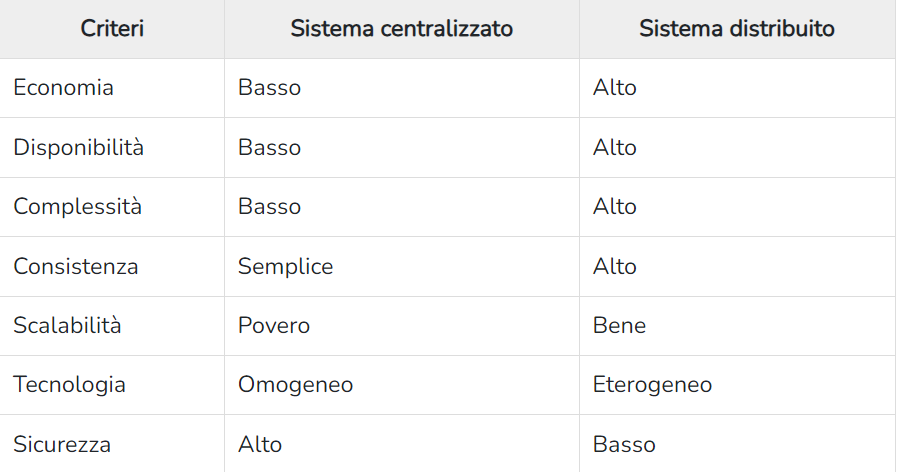
\includegraphics[scale=0.5]{images/central_vs_distribution.png}
    \caption{Confronto tra architetture centralizzate e distribuite}
    
\end{figure}

\section{Apache Druid}
\textbf{Apache Druid} è un database di analisi in tempo reale progettato per analisi rapide, i suoi punti di forza sono le alte prestazioni in esecuzione di query su set di dati di grandi dimensioni.
\textbf{Druid} è comunemente utilizzato come back-end del database per le GUI di applicazioni analitiche o per API altamente simultanee che richiedono aggregazioni veloci. Mostra le sue migliori prestazioni con dati orientati agli eventi.
\subsection{Caratteristiche principali}
\textbf{Druid} combina le idee provenienti da serie temporali e sistema di ricerca, \textit{data-warehouse}.
Le caratteristiche principali sono:
\begin{itemize}
    \item formato di archiviazione a colonne: utilizza una archiviazione orientata alle colonne e carica soltanto le colonne necessarie per una determinata query. Inoltre ottimizza l'archiviazione delle colonne in base al tipo di dato;
    \item sistema distribuito scalabile: le distribuzioni tipiche di Druid si estendono su cluster che vanno da decine a centinaia di server ciò permette di mantenere un tempo di latenza molto basso, al di sotto di pochi secondi;
    \item elaborazione massicciamente parallela: le query vengono elaborate in parallello sull'intero cluster;
    \item injection in tempo reale o batch: \textbf{Druid} è in grado di elaborare sia dati in tempo reale che in batch, i dati acquisiti sono immediatamente disponibili per le successive interrogazioni;
    \item è dotato di un sistema di autobilanciamento e auto individuazione dei guasti:il cluster Druid si riequilibra automaticamente in background senza tempi di inattività, inoltre se un server \textbf{Druid} si guasta, il sistema instrada automaticamente i dati intorno al danno fino alla risoluzione, infatti \textbf{Druid} è progettato per funzionare senza tempi di inattività;
    \item l'architettura nativa del cloud è tollerante ai guasti: \textbf{Druid} archivia in modo sicuro una copia dei tuoi dati in un archivio profondo (in genere su su fyle system o sul cloud), tali dati saranno accessibili semopre anche nel momento in cui i server falliscano; ciò permette l'esecuzione di query anche nei momenti di ripristino.
    \item Indici per filtraggio rapido: \textbf{Druid} utilizza indici bitmap compressi per creare indici che consentano il filtraggio rapido e la ricerca su più colonne;
    \item Partizionamento basato sul tempo: \textbf{Druid} prima suddivide i dati in base al tempo, è possibile in ogni caso aggiungere altri tipi di filtri;
   \item  Algoritmi approssimati:
   \textbf{Druid} permette l'utilizzo di algoritmi offrono un utilizzo limitato della memoria e sono spesso sostanzialmente più veloci dei calcoli esatti, dove sono richiesti conteggi più esatti \textbf{Druid} offre pure questa funzionalità.
   \item Riepilogo automatico al momento dell'acquisizione: \textbf{Druid} supporta facoltativamente il riepilogo dei dati al momento dell'acquisizione.
\end{itemize}

\subsection{Funzionamento}
\subsubsection{DistribuzioniSu singolo nodo}
\textbf{Apache Druid} include molteplici configurazioni su singola macchina si trattano di distribuzioni oramai poco utilizzate.
\\
Esistono configurazioni molto piccole pensate per macchine con poca \textbf{CPU} e \textbf{memoria}, pensate per ambienti con risorse limitate, come i piccoli contenitori \textit{Docker}.
\subsubsection{Distribuzione in cluster}
\textbf{Apache Druid} è progettato per essere distribuito come cluster scalabile e con tolleranza ai guasti.\\
In generale è consigliato andare a creare un cluster che ospita: 
\begin{itemize}
    \item i server principali (Coordinator e Overlord): sono responsabili della gestione dei metadati e delle esigenze di coordinamento del  cluster, possono essere collocati insieme sullo stesso server;
    \item i server dati (Historicals e MiddleManager):
    per gestire i dati effettivi nel tuo cluster,traggono grandi vantaggi da CPU, RAM e SSD;
    \item i server di interrogazione:
    i \textbf{Druid Broker} accettano le richieste e le distribuiscono al resto del cluster, è possibile anche mantenere una cache delle query in memoria.
\end{itemize}
\subsection{L'architettura}
Druid ha un'architettura distribuita progettata per essere compatibile con il cloud. È possibile andare ridimensionare i servizi per avere la massima flessibilità. Inoltre una architettura di questo tipo è maggiormente tollerante ai guasti, un malfunzionamento di una componente non influisce immediatamente sulle altre.
\begin{figure}[h]
    \centering
    \includegraphics[scale=0.5]{images/architettura_druid.png}
    \caption{Architettura Druid}
    \label{fig:my_label}
\end{figure}
\subsection{Servizi offerti}
\subsection{Server principale}
Un server Master gestisce l'ingestion e la disponibilità dei dati: è responsabile dell'avvio di nuovi job di ingestion e del coordinamento della disponibilità dei dati sui "Data server" descritti di seguito.
\subsubsection{Servizio di coordinamento}
Ha il compito di gestire la disponibilità dei dati dei l cluster.
\textbf{Druid Coordinator} comunica ai processi storici di caricare o rilasciare segmenti in base alle configurazioni.
Inoltre è responsabile del caricamento di nuovi segmenti, dell'eliminazione di segmenti obsoleti,della garanzia che i segmenti siano "replicati" (ovvero, caricati su più nodi storici diversi) un numero corretto (configurato) di volte e dello spostamento ("bilanciamento") dei segmenti tra Historical nodi per mantenere quest'ultimo caricato uniformemente.
\textbf{Druid Coordinator} prima di eseguire le varie operazioni valuta lo stato attuale del cluster. Inoltre come gli altri servizzi mantiene una connessione a un cluster \textbf{Zookeeper} per le informazioni sul cluster corrente. Infine il servizio di cooordinamento ha anche una connessione ad un databse contenente l'elenco dei segmenti utilizzati.
\subsubsection{Servizio di Overlord}
 È responsabile dell'accettazione delle attività, del coordinamento della distribuzione delle attività, della creazione di blocchi attorno alle attività e della restituzione degli stati ai chiamanti. È possibile eseguirlo sia in modalità locale, per flussi di lavoro semplici, che remota nella quale occupa uns server dedicato.
 \subsection{Server di interrogazione}
 Un server di query fornisce gli endpoint con cui interagiscono gli utenti e le applicazioni client, instradando le query ai server di dati o ad altri server di query.
 \subsubsection{Servizio Broker}
In un cluster distribuito è il servizio a cui instradare le query. Comprende i metadati forniti da \textbf{Zookeeper}, dove ricavare i dati necessari ad elaborare i risultati delle query.\\
Infine unisce i risultati di tutti i risultati elaborati per fornire un'unica risposta alla query richiesta.
\subsubsection{Servizio di router (opzionale)}
 È il servizio che ha il compito di instradare le query a diversi processi \textbf{Broker}. Le query vengono instradate in base alle regole di caricamento dei segmenti che vengono applicate. Questa configurazione fornisce l'isolamento delle query in modo tale che le query per i dati più importanti non siano influenzate dalle query per i dati meno importanti.
 \subsection{Server dati}
 Un server di dati esegue processi di acquisizione e archivia dati interrogabili.
 \subsubsection{Servizio storico}
 Ogni servizio  copia o estrae i file di segmento da Deep Storage al disco locale in un'area chiamata \textit{segment cache} e rispondono alle domande su tali segmenti.\\Il coordinatore controlla l'assegnazione dei segmenti agli storici e l'equilibrio dei segmenti tra gli storici.  I servizio di storico non comunicano direttamente tra loro, né comunicano direttamente con il Coordinatore. Invece, il coordinatore crea voci temporanee in \textbf{Zookeeper} in un percorso della coda di caricamento . Ogni processo storico mantiene una connessione con \textbf{Zookeeper}, osservando quei percorsi per le informazioni sui segmenti.
\subsubsection{Servizio MiddleManager}
I processi MiddleManager gestiscono l'inserimento di nuovi dati nel cluster. Sono responsabili della lettura da fonti di dati esterne e della pubblicazione di nuovi segmenti Druid.
\subsubsection{Servizio Peone}
I servizzi Peon sono motori di esecuzione delle attività generati dai \textbf{MiddleManager}. Ogni \textbf{Peon} esegue una JVM separata ed è responsabile dell'esecuzione di una singola attività. I Peon girano sempre sullo stesso host del \textbf{MiddleManager} che li ha generati.
\subsubsection{Servizio di indicizzazione}
In alterenativa ai \textbf{MiddleManger} ed ai \textbf{Peon}.\\
Invece di eseguire il fork di processi JVM separati per attività, l'indicizzatore esegue le attività come singoli thread all'interno di un singolo processo JVM.\\
L'indicizzatore è progettato per essere più facile da configurare e distribuire rispetto al sistema MiddleManager + Peon e per consentire una migliore condivisione delle risorse tra le attività. 
\subsection{Deep dive}
\subsubsection{Deep storage}
Il \textbf{deep storage} è dove vengono archiviati i segmenti. È un mceccanismo non fornito da \textbf{Druid}.\\
Fintanto i servizi di \textbf{Druid} possono vedere questa infrastruttura di archiviazione e accedere ai segmenti archiviati su di essa, non  si perdereanno i  dati indipendentemente dal numero di nodi Druid che persi.\\
Il \textbf{deep storage} può essere di due tipi:
\begin{itemize}
    \item locale: destinato ad un solo server o a più server che hanno  acesso ad un filesystem condiviso;
    \item su cloud: è più convenienti, più scalabile e più robuste rispetto all'impostazione di un filesystem condiviso. \textbf{Druid} è compatibile con diveresi sistemi cloud come: Azure, Amazon S3, Google.
\end{itemize}
\subsubsection{Metadata storage}
È l'archivio, basato su dipendeza esterna, dove vengono conservati tutti i metadati essenziali per il funzionamento di un cluster Druid.
Druid utilizza l'archivio dei metadati per ospitare vari metadati sul sistema, ma non per archiviare i dati effettivi.\\
Contiene: 
\begin{itemize}
    \item record di segmenti;
    \item record di regole;
    \item record di configurazione;
    \item registri di controllo.
\end{itemize}
Come servizio predefinito \textbf{Druid} ustilizza \textbf{Derby}, ma archivi più adatti alla produzione sono \textbf{MySQL} e \textbf{PostgreSQL}.
\paragraph{Tabella dei segmenti}
Questa tabella memorizza i metadati sui segmenti che dovrebbero essere disponibili nel sistema (chiamati anche segmenti usati).La tabella viene interrogata dal coordinatore per determinare l'insieme di segmenti che dovrebbero essere disponibili per l'interrogazione nel sistema. La tabella ha due colonne funzionali principali, le altre colonne sono a scopo di indicizzazione.\\
Il primo valore \textbf{used} indica che il segmento deve essere utilizzato dal cluster, è il mezzo attraverso cui si caricano e scaricano i segmenti dal cluster senza rimuovere i metadati.\\
La seconda è la  \textbf{payload} che archivia un BLOB JSON che contiene tutti i metadati per il segmento.
\paragraph{Tabella delle regole}
È la tabella che memorizza le varie regole su dove allocare e deallocare i segmenti del cluster.
\paragraph{Tabella di configurazione}
Hanno los copo di memorizzare  gli oggetti di configurazione di runtime.\\
In futuro avranno lo scopo di modificare alcuni parametri di configurazione nel cluster in fase di esecuzione.
\paragraph{Tabella delle attività}
Si riferiscono alle tabelle create e gestite dall'\textbf{Overlord} e \textbf{MiddleManager}.
\paragraph{Tabella di revisione}
È la tabella che memorizza le modifiche apportate alla configurazione.\\
Hanno accesso hai metadati solo: il servizio di indicizzazione, il servizio in tempo reale e il servizio di coordinamento.
\subsubsection{Zookeeper}
\textbf{Apache Druid} utilizza \textbf{Apache ZooKeeper} per la gestione dello stato corrente del cluster.\\
In \textbf{Zookeeper} avengono le seguenti attività: 
\begin{itemize}
    \item Elezione del servizio di coordinamento;
    \item Protocollo di "pubblicazione" del segmento degli storici;
    \item Protocollo di caricamento/rilascio del segmento tra Coordinatore e Storico;
    \item elezione del servizio di \textbf{Overlord};
    \item Gestione delle attività di \textbf{Overlord e MiddleManager};
    
\end{itemize}

\subsection{Archiviazione dei dati}
I dati in\textbf{Apache Druid} vengono archiviati in \textit{datasources} tabelle simili a quelle utilizzate dai database relazionali. Ogni tabella viene partizionata in base agli intervalli di tempo. Ogni intervallo di tempo è chiamato blocco. All'interno di un blocco, i dati vengono partizionati in uno o più segmenti . Ogni segmento è un singolo file, che in genere comprende fino a pochi milioni di righe di dati. Si può pensare che i segmenti dati è come vivano in una sequenza temporale.\\
Ogni segmento viene creato da un \textbf{MiddleManager} come mutable e uncommitted.  I dati sono interrogabili non appena vengono aggiunti a un segmento senza commit.\\
Il processo di creazione del segmento accelera le query successive producendo un file di dati compatto e indicizzato. \\
Periodicamente i segmenti vengono sottoposti a commit e pubblicati in deep storage diventano immutabili e passano dai MiddleManager ai processi storici. Inoltre nell'archivio dei metadati viene scritta una voce al segmento che lo descrive.\\
Tali informazioni inidicano al coordinatore quali dati sono presenti nel cluster.

\subsection{I segmenti}
\textbf{Apache Druid} memorizza i suoi dati e indici in file di segmenti partizionati in base al tempo.
\textbf{Druid} crea un segmento per ogni intervallo di segmento che contiene dati.
Affinchè \textbf{Druid} funzioni bene  con un carico di query elevato, è importante che la dimensione del file del segmento rientri nell'intervallo consigliato di 300-700 MB. Se questo non accade si può valutare la possibilità di modifica della granularità dell'intervallo di tempo del segmento.
\subsubsection{Struttura del file di segmento}
I file di segmento sono colonnari : i dati per ciascuna colonna sono disposti in strutture di dati separate. Memorizzando ciascuna colonna separatamente, Druid riduce la latenza delle query analizzando solo le colonne effettivamente necessarie per una query. \\
Una volta che una query identifica le righe da selezionare, le decomprime, estrae le righe pertinenti e applica l'operatore di aggregazione desiderato.  Se una query non richiede una colonna, Druid ignora i dati di quella colonna.
Le colonne di tìpo dimension supportano le operazioni di filtro e raggrupamento, quindi richiede l'utilizzo delle seguenti tre strutture dati: 
\begin{itemize}
    \item Dizionario : esegue il mapping dei valori agli ID interi, consentendo una rappresentazione compatta dell'elenco e dei valori bitmap;
    \item List : i valori della colonna, codificati utilizzando il dizionario.
    Questi operatori consentono l'esecuzione di query che aggregano esclusivamente metriche basate su filtri senza accedere all'elenco di valori.
    \item Bitmap : una bitmap per ogni valore distinto nella colonna, per indicare quali righe contengono tale valore.
\end{itemize}
Per ogni riga nell'elenco dei dati della colonna, esiste solo una singola bitmap con una voce diversa da zero. Ciò significa che le colonne con cardinalità elevata hanno bitmap estremamente rade e quindi altamente comprimibili. 
\subsubsection{L'identificazione del segmento}
Gli identificatori di segmento in genere contengono l'origine dati del segmento, l'ora di inizio dell'intervallo (in formato ISO 8601 yyyy-mm-gg), l'ora di fine dell'intervallo (in formato ISO 8601 yyyy-mm-gg) e le informazioni sulla versione. Se i dati vengono ulteriormente partizionati oltre un intervallo di tempo, l'identificatore di segmento contiene anche un numero di partizione.
\subsubsection{Indicizzazione e consegna del segmento}
L'\textbf{indicizzazione} è il meccanismo mediante il quale vengono creati nuovi segmenti e l'\textbf{handoff} è il meccanismo mediante il quale vengono pubblicati e iniziano a essere serviti dai processi storici. \\
Un'attività di indicizzazione viene avviata e crea un nuovo segmento. Deve determinare l'identificatore del segmento prima di iniziare a costruirlo.\\ L'attività di aggiunta di un nuovo segmento viene fatta chiamando un'API di "allocazione" su \textbf{Overlord} per aggiungere potenzialmente una nuova partizione a un set di segmenti esistente.  Per un'attività che sta sovrascrivendo (come un'attività Hadoop o un'attività di indicizzazione non in modalità di aggiunta), questa operazione viene eseguita bloccando un intervallo e creando un nuovo numero di versione e un nuovo set di segmenti.\\
Da questo momento in poi il segmento è interrogabile e quando l'attività di indicizzazione ha terminato li inserisce nello deep storage  e li pubblica scrivendolo nell'archivio dei metadati. Per i processi in real-time, per garantire la disponibilità dei dati attende il caricamento dei dati.
\subsubsection{Indentificatore di segmento}
Tutti i segmenti hanno un identificatore in quattro parti con i seguenti componenti:
\begin{itemize}
    \item nome dell'origine dati;
    \item intervallo di tempo;
    \item numero di versione;
    \item numero di partizione.
\end{itemize}
\subsubsection{Versione del segmento}
Il numero di versione fornisce una forma di controllo della concorrenza multi-versione (MVCC) per supportare la sovrascrittura in modalità batch. Il passaggio da una versione all'altra dal lato utente non è percepibile,  perché Druid lo gestisce caricando prima i nuovi dati e non appena i nuovi dati sono stati caricati, cambiando tutte le nuove query per utilizzare quelle nuovi segmenti. Quindi rilascia i vecchi segmenti pochi minuti dopo. 
\subsubsection{Ciclo di vita del segmento}
Ogni segmento ha un ciclo di vita che coinvolge le seguenti tre aree principali:
\begin{itemize}
    \item archivio dei metadati: contiene i metadati del segmento e vengono archiviati nell'archivio dei metadati una volta terminata la costruzione di un segmento.
    \item Archiviazione profonda: i file di dati del segmento vengono inseriti nell'archiviazione profonda una volta terminata la costruzione di un segmento. Ciò avviene immediatamente prima della pubblicazione dei metadati nell'archivio dei metadati.
    \item Disponibilità per l'interrogazione: i segmenti sono disponibili per l'interrogazione su alcuni server di dati Druid, come un'attività in tempo reale o un processo storico.
\end{itemize}
\pagebreak
\subsubsection{Injection dei dati}
 I principali metodi di ingestione di Druid sono tutti basati su pull e offrono garanzie transazionali (verrà caricato o tutto o niente).
 \begin{itemize}
    \item Metodi di ingestione "seekable-stream" supervisionati come Kafka e Kinesis . Con questi metodi, Druid esegue il commit degli offset del flusso nel proprio archivio di metadati insieme ai metadati del segmento, nella stessa transazione, in questo caso \textbf{Apache Druid}  pubblica i segmenti prima che tutti i dati per un blocco temporale siano stati ricevuti;
    \item Inserimento batch basato su Hadoop; Ogni attività pubblica tutti i metadati del segmento in un'unica transazione. 
    \item Importazione batch nativa . In modalità parallela, l'attività del supervisore pubblica tutti i metadati del segmento in un'unica transazione al termine delle attività secondarie.
 \end{itemize}
\subsection{Casi d'uso}
\subsubsection{Potenza di analisi dati in real-time e applicazioni dati}
Un caso d'uso importante per \textbf{Apache Druid} è l'impiego di sistemi di acquisizione dati in tempo reale, query rapide e tempo di attività. \textbf{Druid} viene utilizzato per alimentare GUI per applicazioni analitiche o per \textbf{API} simultanee che necessitano di aggregazioni veloci. Funziona meglio su dati orientati agli eventi.
Le aree di impiego più comuni:
\begin{itemize}
    \item analisi dei flussi di clic
    \item analisi della telemetria di rete (monitoraggio delle prestazioni della rete)
    \item archiviazione delle metriche del server
    \item metriche delle prestazioni dell'applicazione
    \item operazioni \textbf{OLAP}
\end{itemize}
\subsubsection{Attività e comportamento dell'utente}
\textbf{Apache Druid} viene speso utilizzato per effettuare misurazioni sul coinvogimento degli utenti e il monitoraggio dei dati di test. \\
È utilizzato per calcolare metriche utente come conteggi distinti sia esattamente che approssimativamente.
\subsubsection{Flussi di rete}
Druid è comunemente usato per raccogliere e analizzare i flussi di rete. Druid viene utilizzato per  suddividere arbitrariamente i dati del flusso lungo qualsiasi insieme di attributi.
Questi attributi includono spesso attributi di base come IP e porta.\textbf{Druid} permette di gestire schemi flessibili di attributi.
\subsubsection{Marketing digitale}
\textbf{Druid} viene comunemente usato per archiviare e interrogare i dati pubblicitari online. Questi dati in genere provengono dagli ad server e sono fondamentali per misurare e comprendere le prestazioni delle campagne pubblicitarie, le percentuali di clic, i tassi di conversione (tassi di abbandono) e molto altro. In generale \textbf{Druid} è stato creato per gestire questo tipo di dati in grandi dimensioni.\\
Inoltre \textbf{Druid} può calcolare una serie di altre metriche per calcolare tendenze su grandi moli id dati.
\subsubsection{Gestione delle prestazioni dell'applicazione}
Druid viene spesso utilizzato per tenere traccia dei dati operativi generati dalle applicazioni.
Similmente all'analisi dell'attività utente, in questo caso le metriche calcolate, o stimaste riguardano dati emessi dall'applicazione stessa.
\subsubsection{Metriche IoT e dispositivi}
\textbf{Druid} può essere utilizzato acquisire i dati generati dalla macchina in tempo reale ed eseguire rapide analisi ad hoc per misurare le prestazioni, ottimizzare le risorse hardware o identificare i problemi.\\
A differenza di altri database di serie temporali, \textbf{Druid} fornisce una serie di funzionalità di ricerca e parrtizionamento che gli permette di eseguire query molto velocemente.
\subsubsection{Operazioni OLAP}
\textbf{Apache Druid} viene utilizzato per accelerare l'esecuzione di query e potenziare le applicazioni. È progettato per un'elevata concorrenza e query in meno di un secondo, alimentando l'esplorazione interattiva dei dati attraverso un'interfaccia utente. Ciò fornisce una migliore soluzione interattiva con l'utente. Permette di effettuare analisi interattive su garbdi moli di dati.
\subsection{Modello dei dati}
Druid memorizza i dati in \textit{datasources} molto simili alle tabelle di un tradizionale database relazione e alle serie temporali.
Il modello di dati di \textbf{Druid} presenta essenzialmnente le seguenti componenti:
\begin{itemize}
    \item Timestamp principale: Gli schemi Druid devono sempre includere un timestamp primario. Viene utilizzato per partizionare ed ordinare i dati. Inoltre il timestamp viene utilizzato per recuperare rapidamente i dati all'interno di un detrminato intervallo di tempo.
    \item Dimension: sono colonne che Druid memorizza "così come sono". Si possono utilizzare per qualsiasi scopo: filtrare, applicare aggregatori e così via.
    \item Metrics: sono colonne che Druid archivia in forma aggregata e diventano più utili se attivi il rollup è una forma di aggregazione che comprime le dimensioni mentre aggrega i valori nelle metriche, ovvero comprime le righe ma conserva le informazioni di riepilogo.
\end{itemize}
\pagebreak
\subsubsection{Metrica}
Le metriche sono colonne che \textbf{Druid} archivia in forma aggregata. Le metriche sono più utili quando abiliti il \textbf{rollup}.\\ 
Se specifichi una metrica, puoi applicare una funzione di aggregazione a ogni riga durante l'importazione.
Il rollup è una forma di aggregazione che combina più righe con lo stesso valore di timestamp e gli stessi valori di dimensione; mentre aggrega i valori nelle metriche, ovvero comprime le righe ma conserva le informazioni di riepilogo.
\subsubsection{Dimension}
Le dimensioni sono colonne che Druid memorizza "così come sono". Le dimensioni possono essere utilizzzate per qualsiasi scopo. Ad esempio per  raggruppare, filtrare o applicare aggregatori alle dimensioni in fase di query, se necessario. Se il \textbf{rollup} è disabilitato le dimension vengono trattate come colonne da importare.
\subsection{Schema design tips}
\begin{itemize}
   

 \item nell'importazione dei dati \textbf{Druid} con o senza rollup: aggregando parzialmente i tuoi dati durante l'importazione, riducendo potenzialmente il numero di righe, diminuendo l'impronta di archiviazione e migliorando le prestazioni delle query. Mentre senza rollup \textbf{Druid} archivia una riga per ogni riga di input.
 \item ogni riga in Druid deve avere un timestamp, tale informazione potrà essere utilizzata per successivi grappamenti.
 \item tutte le colonne del modello di archiviazione di     \textbf{Druid} sono metriche ad eccezione del timestamp
 \item le colonne dimensione vengono archiviate così come sono
 \item le colonne delle metriche vengono archiviate preaggregate , quindi possono essere aggregate solo al momento della query.
\end{itemize}
\subsubsection{Modello relazionale}
In \textbf{Druid} in generale le \textit{datasources} sono molto simili alle tabelle utilizzate nel modelli relazionali ma in questo caso si preferisce creare tabelle che permettano elaborazioni piatte: recupero delle informazioni senza l'utilizzo di join tra tabelle, ciò consente un aumento delle prestazioni.
\subsubsection{Modello su serie storiche}
Simile ai database delle serie temporali, il modello di dati di Druid richiede un timestamp. Druid non è un database di serie temporali, ma è una scelta naturale per l'archiviazione di dati di serie temporali. Il suo modello di dati flessibile consente di archiviare sia dati di serie temporali che non, anche nella stessa origine dati.\\
Per ottenere prestazioni ottimali di compressione e query in Druid per i dati delle serie temporali, è importante partizionare e ordinare in base al nome della metrica, come fanno spesso i database delle serie temporali.
\subsubsection{Utilizzo degli Sketches}
Nel momento in cui si vanno ad inserire dati \textbf{Druid} non li memorizza direttamente uno Sketche che poi può inserire nell'esecuzione delle query successive. \\Ogni Sketche può essere acquisito dall'esterno di Druid o creato da dati grezzi al momento dell'acquisizione. È progettato per un solo particolare tipo di calcolo. In questo modo si riduce il \textbf{rollup} e si riduce la memoria utilizzata in fase di query.
\subsubsection{Utilizzo del timestamp}
Gli schemi \textbf{Druid} devono sempre includere un timestamp primario. Il timestamp principale viene utilizzato per partizionare e ordinare i dati, quindi dovrebbe essere il timestamp su cui filtrerai più spesso. Druid è in grado di identificare e recuperare rapidamente i dati corrispondenti agli intervalli di tempo della colonna timestamp primaria.
Se lo schema lo richiede è possibile importare anche timestamp secondari.
\subsubsection{Autorillevamento del tipo}
È possibile fare in modo che \textbf{Druid} deduca lo schema e i tipi per i tuoi dati parzialmente o completamente impostando. \\
Nella deduzione del tipo \textbf{Druid} sceglie il tipo nativo più appropiato.\\
Per le colonne di tipo misto vengono archiviate nel tipo meno restrittivo che può rappresentare tutti i valori nella colonna.
\subsection{Data rollup}\label{subsection:rollup}
Al momento dell'acquisizione dei dati \textbf{Apache Druid} può eseguire operazioni di raggrupamento sui dati per ridurre la quantità di dati grezzi da archiviare. \\
Da questo punto di vista il \textbf{rollup} non è altro che una forma di riepilogo e preaggregamento dei dati finalizzato a ridurre lìordine di grandezza delle righe da archiviare.\\
Il \textbf{rollup} se da un lato porta una riduzione drastica degli eventi da analizzare, dall'altro non permette più di interrogare i singoli eventi.\\
Al momento dell'\textbf{injection} il \textbf{rollup} è abilitato di default: \textbf{Apache Druid} raggrupa in automatico gli eventi caratterizzati da stesso valore di \textbf{timestamp} e stesso valore per le \textbf{Dimension}. \\
Se il \textbf{rollup} è disabilitato, \textbf{Apache Druid} caricherà gli eventi così come sono stati generati.senza alcun riepilogo.
\subsubsection{Casi d'uso}
È convenienete andare ad utilizzare il \textbf{rollup} se si desiderano prestazioni ottimali e vicoli di spazio rigorosi o quando non si ha necessità di avere a disposizione dati grezzi con alta cadrdianlità. \\
Mentre se si ha bisogno di risultati per righe, l'utilizzo del \textbf{rollup} non è la scelta più adatta; è necessario in quel caso efettuare delle operazionui di \textbf{GROUP BY} a query time.
\\
In ogni caso, per soddisfare entrambi i casi d'uso appena citati è possibile andare a configurare 2 datasource: uno con \textbf{rollup} attivo, con il riepilogo degli eventi generati, e uno con \textbf{rollup} disabilitato contenente tutti i dati grezzi.
\subsubsection{Tipi di rollup}
A seconda del metodo di importazione, \textbf{Apache Druid} presenta due metodi differenti di \textbf{rollup}.
\begin{itemize}
    \item rollup perfetto: \textbf{Apache Druid} aggrega perefettamenete i dati a injection time;
    \item Best-effort rollup: \textbf{Apache Druid} potrebbe non riuscire ad aggregare perfettamente di input pertanto si potrebbe verificare che più segmenti dati contengano dati con stesso timestamp e stesso valore di Dimension.
\end{itemize}
In generale I metodi di inserimento che garantiscono un rollup perfetto utilizzano un ulteriore passaggio di pre-elaborazione per determinare gli intervalli e il partizionamento prima dell'inserimento dei dati. Questa fase di pre-elaborazione esegue la scansione dell'intero set di dati di input. Anche se questo passaggio aumenta il tempo necessario per l'inserimento, fornisce le informazioni necessarie per un rollup perfetto.\\
Mentre i metodi che garantiscono il \textbf{Best-effort rollup} lo fanno per i seguenti motivi: 
\begin{itemize}
    \item la parallelizzazione dell'inserimento avviene senza un passaggio di mescolamento necessario per il \textbf{rollup} perfetto;
    \item Il metodo di importazione utilizza la pubblicazione incrementale , il che significa che finalizza e pubblica i segmenti prima che tutti i dati per un blocco temporale siano stati ricevuti, tutti i tipi di importazione di streaming vengono eseguiti in questa modalità.
\end{itemize}
\subsection{Le lookups}
In \textbf{Apache Druid} le \textbf{lookup} sono una funzionalità che consentono di sostituire i valori delle \textbf{Dimension} con nuovi valori. Tale cocetto può essere paragonato alla unione di tabelle in un \textbf{data warehouse}.\\
Le tabelle di \textbf{lookup} sono costituite da un campo \textbf{chiave} a cui viene associato un campo \textbf{valore} che andrà a sostituire la chiave.\\
Le tabelle di \textbf{lookup} non hanno cronologia e lavorano indipendentemente dall'intervallo di tempo. su cui si esegue la query: restituiscono sempre il dato corrente.
\subsubsection{Sintassi SQL di query con l'utilizzo delle tabelle di lookup}
In \textbf{Apache Druid} le tabelle di \textbf{lookup} possono essere utilizzate attraverso funzione\\ $LOOKUP(keys,lookup\_table\_name)$.
\begin{lstlisting}[language=SQL,showstringspaces=false,]
SELECT LOOKUP(store, 'store_to_country') AS country, SUM(revenue)
FROM sales
GROUP BY 1
\end{lstlisting}
Le tabelle di \textbf{lookup} consentendo le operazione di tipo join.
\begin{lstlisting}[language=SQL,showstringspaces=false,]
SELECT store_to_country.v AS country, SUM(sales.revenue) AS country_revenue
FROM sales INNER JOIN lookup.store_to_country ON sales.store = store_to_country.k
GROUP BY 1
\end{lstlisting}
\subsubsection{Tipi di lookup}
In generale le tabelle di \textbf{lookup} possono essere di due tipi: iniettive e non iniettive. \\
Nel primo tipo rietrano tutti i casi d'uso legati alla mappatura univoca tra chiave e valore; mentre nel secondo caso rientrano tutte le mappature nelle quali più chiavi riferiscono lo stesso valore.\\
Nel momento in cui si creano tabelle di \textbf{lookup} iniettive \textbf{Apache Druid} è in grado di applicare ulteriori ottimizzazioni nella esecuzione delle query.
\\Tale fatto deve essere tenuto in considerazione nel caso di aggregazioni, in quanto, nel caso in cui chiavi diverse puntino allo stesso valore (tabella di \textbf{lookup} non iniettiva), nel risultato di una query comparirano due valori che avrebbero dovuto essere aggregati.
\subsubsection{Casi d'uso}
Le tabelle di \textbf{lookup} sono particolarmente utili nei processi di \textbf{Data enrichment}.\\
Inoltre posssono andare a risolvere anche essere una possibile soluzione al problema degli aggiornamenti. In questo caso ogni aggiornamento di stato viene visto come un nuovo evento e viene aggiunto al \textbf{datasource} originale.\\
Per estrarre sempre il dato più recente si utilizza una \textbf{lookup} iniettiva che mappa ogni chiave con il valore dell'attributo richiesto. Essendo le tabelle di \textbf{lookup} indipendenti dagli intervalli temporali, verrà reatsituito il valore più recente. 
\subsection{Confronto Apache Druid e PostgreSQL}
Per andare ad eveidenziare pregi e diffetti di \textbf{Apache Druid} è stato scelto di confrontarlo con un database relazionale come \textbf{PostgreSQL}, nella esecuzione di query su un dataset di 1 milione di righe.\\
Il test effettuato non usufruisce della cache.\\
Lo schema logico del dataset è il seguente:
\begin{lstlisting}[language=SQL]
    CREATE TABLE transazione
(
    __time timestamp,
    cliente text,
    prodotto text,
    quantita int,
    gradimento int
)

\end{lstlisting}

\subsubsection{Query}
\begin{lstlisting}[language=SQL]
    query1: 
    SELECT * FROM transazione
    query2: 
    SELECT DATA_TRUNC('MINUTE',__time), cliente, prodotto, COUNT(*) 
    FROM transazione 
    WHERE gradimento>3 
    GROUP BY DATA_TRUNC('MINUTE',__time), cliente, prodotto
    query3: 
    SELECT DATA_TRUNC('HOUR',__time), cliente, prodotto, gradimento 
    FROM transazione 
    WHERE gradimento>3 
    GROUP BY DATA_TRUNC('HOUR',__time), cliente, prodotto, gradimento
\end{lstlisting}
\begin{center}
    \begin{tblr}{
  colspec={XXX},
  row{odd}={bg=lightgray},  
  row{1}={bg=black,fg=white},
}
\centering
  & \centering Apache Druid [s] & \centering PostgreSQL [s] \\\hline 
  \centering
  query1 &  \centering 0.007  & \centering 0.77 \\ \hline
  \centering
  query2 &  \centering 0.45 &  \centering 0.57 \\ \hline 
  \centering
  query3 & \centering 0.30 & \centering 0.60 \\ \hline
  \end{tblr}
\end{center}
\section{Kubernetes}
\subsection{Panoramica e caratteristiche principali}
\textbf{Kubernetes} è una piattaforma open source utilizzata per l'orchestrazione e la gestione dei nodi.\\
Il nome Kubernetes deriva dal greco, significa timoniere o pilota. \\
È un servizio estendibile per la gestione di carichi di lavoro e servizi containerizzati. Presenta un grande ecosistema in rapida crescita. \\

\subsection{Casi d'uso}
I container sono un buon modo per raggruppare ed eseguire le applicazioni. In un ambiente di produzione, è necessario gestire i container ed assicurarsi che vi siano tempi di inattività. In tali casi entra in gioco \textbf{Kubernetes} che fornisce un \textbf{framework} finalizzato alla esecuzione di sistemi distribuiti in modo resiliente. \\
\subsection{Funzionalità}
\textbf{Kubernetes} fornisce le seguenti funzionalità:
\begin{itemize}
    \item \textbf{rilevamento dei servizi e bilanciamento del carico}: \textbf{Kubernetes} è in grado di bilanciare il carico e distribuire il traffico di rete in modo che la distribuzione sia stabile;
    \item \textbf{orchestrazione dello storage}: \textbf{Kubernetes} consente di montare storage locali, provider di cloud pubblico e altro;
    \item \textbf{rollout e rollback automatizzati}: puoi descrivere lo stato desiderato per i tuoi container distribuiti utilizzando Kubernetes e può cambiare lo stato effettivo nello stato desiderato a una velocità controllata.
    \item \textbf{bin packing automatico}: è possibile impartire a \textbf{Kubernetes} quanta CPU e memoria (RAM) ha bisogno ogni container; inoltre \textbf{Kubernetes} può adattare i container ai tuoi nodi per utilizzare al meglio le tue risorse;
    \item \textbf{riparazione automatica}: \textbf{Kubernetes} è in grado di rillevare i container che hanno avuto esito negativo, sotituirli e terminare i container non rispondono allo stato definito dall'utente;
    \item \textbf{gestione dei secrets e della configurazione}: \textbf{Kubernetes} ti consente di archiviare e gestire informazioni riservate 
\end{itemize}
\subsection{Architettura}
\textbf{Kubernetes} viene distribuito in un cluster. \\
Un cluster è costituito da un insiemee di macchine \textbf{worker}, denominate nodi, che eseguono le applicazioni containerizzate. Ogni cluster ha almeno un nodo \textbf{worker}.\\
I nodi \textbf{worker} ospitano i \textbf{POD} che rappresentano i componenti di lavoro dell'applicazione. Il \textbf{control pane} gestisce i nodi di lavoro e i \textbf{POD} del cluster. In ambienti di produzione per garantire tolleranza ai guasti e alta disponibilità il \textbf{control pane} e \textbf{POD} sono eseguiti su più calcolatori e un cluster esegue i nodi. 
\subsubsection{I componenti del control pane}
I componenti di \textbf{control pane} prendono decisioni globali sul cluster, oltre a rispondere ad eventi del cluster. Per semplicità i componenti di \textbf{control pane} vengono tutti eseguiti sulla stessa macchina.
\paragraph{kube-apiserver}
È un componente del \textbf{control pane} di  \textbf{Kubernetes} che espone l'\textbf{API Kubernetes}. L'implementazione principale è un \textbf{kube-apiserver}, progettato per scalare orrizontalmente, distribuendosi su più istanze. È possibile andare a bilanciare il traffico tra tali istanze. 
\paragraph{ecc}
È l'archivio di valore chiave coerente utilizzato come archivio di backup di \textbf{Kubernetes} per tutti i dati del cluster.
\paragraph{kube-scheduler}
È un componente del \textbf{control pane} a cui è affidato il compito di controllare la creazione dei \textbf{POD} senza assegnare nodi su cui eseguirli.\\
Per prendere le decisioni di pianificazione vengono presi incosiderazione i seguenti fattori: 
\begin{itemize}
    \item requisiti di risorse individuali e collettivi;
    \item  vincoli hardware/software/policy;
    \item specifiche di affinità e anti-affinità;
    \item località dei dati;
    \item  interferenza tra carichi di lavoro e scadenze.
\end{itemize}
\paragraph{kube-controller-manager}
È il componente adibito al controllo dei processi. \\
Logicamente ogni \textbf{controller} è un processo separato, ma per ridurre la complessità, sono tutti compilati in un unico binario ed eseguiti in un unico processo.
\paragraph{cloud-controller-manager}
È il componente che incorpora la logica di controllo specifica del cloud. Il \textbf{cloud-controller-manager} consente di collegare il cluster con l'\textbf{API} del provider cloud; separa i componenti che interagiscono con quella piattaforma cloud dai componenti che interagiscono solo con il tuo cluster. Se esegui \textbf{Kubernetes} nei tuoi locali, il cluster non dispone di un \textbf{cloud-controller-manager}.
\subsubsection{I componenti del nodo}
I componenti del nodo vengono eseguiti su ogni nodo, mantenendo i pod in esecuzione e fornendo l'ambiente di runtime \textbf{Kubernetes}.
\paragraph{kubelet}
È un agente che viene eseguito per ogni nodo del cluster e si assicura che i container stiamo eseguendo un \textbf{POD}.
\paragraph{kube-proxy} È un proxy di rete che viene eseguito su ogni nodo del cluster, implementando parte del servizio \textbf{Kubernetes}. Mantiene le regole di rete sui nodi. Queste regole di rete consentono la comunicazione di rete ai \textbf{POD} dalle sessioni di rete all'interno o all'esterno del tuo cluster.
\subsection{Il funzionamento}
\textbf{Kubernetes} esegue i compiti assegnati di lavoro inserendo i container nei \textbf{POD}  per l'esecuzione sui nodi. Un nodo può essere una macchina virtuale o fisica, a seconda del cluster. \\
Ogni nodo è gestito da un \textbf{control pane} e contiene i servizi necessari per l'esecuzione di un \textbf{POD}. I componenti su un nodo includono  il \textbf{kubelet}, un runtime del container, e il \textbf{kube-proxy}.\\
Esistono due modi principali  per aggiungere i nodi: \textbf{Server API} 
\begin{itemize}
    \item il kubelet su un nodo si registra automaticamente nel piano di controllo;
    \item viene aggiunto manualmente un oggetto di tipo \textbf{Node}.
\end{itemize}
Una volta effettuata la creazione dell'oggetto Nodo o il \textbf{kubelet} su un nodo, il \textbf{control pane} che il nuovo oggetto di tipo \textbf{Node} sia integro ( (ovvero tutti i servizi necessari sono in esecuzione, idoneo ad eseguire un POD). \\
Un esempio di configurazione di un nodo, in formato Json può essere il seguente: 
\begin{lstlisting}
{
  "kind": "Node",
  "apiVersion": "v1",
  "metadata": {
    "name": "10.240.79.157",
    "labels": {
      "name": "my-first-k8s-node"
    }
  }
}
\end{lstlisting}
\subsubsection{Unicità del nodo}
Il nome identifica in modo univoco un nodo. Due nodi non possono avere lo stesso nome, perchè \textbf{Kubernetes} presuppone che due risorse con lo stesso nome rappresentino la stessa risorsa. Se tale condizione non venisse rispettata si verificherebbero delle incoerenze di stato dei nodi. \\
\textbf{Se il nodo deve essere sostituito o aggiornato in modo significativo, l'oggetto nodo esistente deve essere prima rimosso dal server API e aggiunto nuovamente dopo l'aggiornamento}.
\subsubsection{Lo stato di un nodo}
Lo stato di un nodo contiene le seguenti informazioni:
\begin{itemize}
    \item Indirizzi: contiene le informazioni: \begin{itemize}
        \item \textbf{HostName}: il nome host riportato dal kernel del nodo;
        \item \textbf{ExternalIP}: in genere l'indirizzo IP del nodo che è instradabile esternamente;
        \item \textbf{InternalIP}: in genere l'indirizzo IP del nodo che è instradabile solo all'interno del cluster.
    \item le conditions: campo che descrivi lo stato di tutti i nodi attivi;
        \begin{itemize}
            \item \textbf{Ready}: Truese il nodo è integro e pronto ad accettare pod, Falsese il nodo non è integro e non accetta pod e Unknownse il controller del nodo non ha ricevuto notizie dal nodo nell'ultimi 40 secondi; 
            \item \textbf{DiskPressure}: True se la capacità del disco è bassa;
            \item \textbf{MemoryPressure}: True se la memoria del nodo è bassa;
            \item \textbf{PIDPressure}: True se ci sono troppi processi sul nodo;
            \item \textbf{NetworkUnavailable}: True se la rete per il nodo non è configurata correttamente.
        \end{itemize}
    \end{itemize}
\end{itemize}
\subsection{Heartbeats}
Gli \textbf{Heartbeats} o battiti del cuore  aiutano il tuo cluster a determinare la disponibilità di ciascun nodo e ad agire quando vengono rilevati errori.\\
Per i nodi ci sono 2 forme di battiti del cuore: 
\begin{itemize}
    \item aggiornamenti al
    $.status$ di un nodo;
    \item allocare oggetti all'interno del $kube-node-lease$ spazio dei nomi; ogni nodo ha un oggetto \textbf{Lease} associato;
\end{itemize}
Rispetto agli aggiornamenti $.status$ di un nodo, un lease è una risorsa leggera. L'utilizzo dei lease per gli heartbeat riduce l'impatto sulle prestazioni di questi aggiornamenti per i cluster di grandi dimensioni.\\
Il \textbf{kubelet} è responsabile della creazione e dell'aggiornamento dei $.status nodi$ e dell'aggiornamento dei relativi $lease$.\\\\\\\\
In particolare si occupa di: 
\begin{itemize}
    \item  aggiorna il nodo $.status$ quando c'è un cambiamento di stato o se non c'è stato alcun aggiornamento per un intervallo configurato (l'intervallo prededfinito è di 5 minuti);
    \item Il \textbf{kubelet} crea e quindi aggiorna il suo oggetto \textbf{Lease} ogni 10 secondi; gli aggiornamenti del \textbf{Lease} si verificano indipendentemente dagli aggiornamenti del \textbf{Lease}.
\end{itemize}
\subsection{Il controllore del nodo}
È un componente del \textbf{control pane} che gestisce i vari aspetti del nodo. \\
I compiti che svolge il controllore sono: 
\begin{itemize}
    \item assegnare un blocco CIDR al nodo quando è registrato;
    \item mantenere aggiornato l'elenco interno dei nodi del controller del nodo con l'elenco delle macchine disponibili del fornitore di servizi cloud;
    \item monitora la salute dei nodi.
\end{itemize}
Per impostazione predefinita, il controller del nodo controlla lo stato di ciascun nodo ogni 5 secondi. 
\subsection{L'elezione del capo}
\textbf{Kubernetes} utilizza anche i \textbf{lease} per garantire che solo un'istanza di un componente sia in esecuzione in un dato momento. 
\subsection{Garbage Collection}
Con \textbf{Garbage Collection} si va ad intendere tutti i meccanismi che \textbf{Kubernetes} utilizza per ripulire le risorse del cluster.\\
Molti oggetti di \textbf{Kubernetes} utilizzano l'\textbf{owner references}, che indicano al \textbf{control pane} quali oggetti dipendono da altri. \textbf{Kubernetes} elimina tutte le risorse correlate ad un oggetto prima di eliminare quest'ultimo.
\subsection{Foreground cascading deletion}
\textbf{Kubernetes} controlla ed elimina gli oggetti che non hanno più riferimenti al proprietario. Quando elimini un oggetto, puoi controllare se Kubernetes elimina automaticamente i dipendenti dell'oggetto, in un processo chiamato eliminazione a cascata. \\
Esistono due tipi di eliminazione a cascata:
\begin{itemize}
    \item Eliminazione a cascata in primo piano: l'oggetto in questione entra in una fase di "eliminazione in corso", L'oggetto rimane visibile tramite l'API \textbf{Kubernetes} fino al completamento del processo di eliminazione;
    \item Eliminazione a cascata in background: il server \textbf{API Kubernetes} elimina immediatamente l'oggetto proprietario e il controller pulisce gli oggetti dipendenti in background. Quando Kubernetes elimina un oggetto proprietario, i dipendenti rimasti vengono chiamati oggetti orfani.
\end{itemize} 
\subsection{Configurazione}
In questa sezione viene descritto come eseguire un'app d'esempio su \textbf{Kubernetes}.\\
Tale esempio presuppone l'esecuzione su singola macchina del cluster e l'utilizzo di \textbf{minikube}.\\
Gli obbiettivi della seguente demo di esempio sono: 
\begin{itemize}
    \item distribuire un'applicazione di esempio su \textbf{minikube};
    \item eseguire l'applicazione;
    \item visualizzare i registri dell'applicazione.
\end{itemize}
\subsubsection{Svolgimento}
Prima di tutto assicurarsi di aver configurato \textbf{minikube} sulla propria macchina. \\
L'installazione può essere effetuata attareverso i seguenti comandi: 
\begin{lstlisting}
curl -LO https://storage.googleapis.com/minikube/releases/latest/minikube-linux-amd64
sudo install minikube-linux-amd64 /usr/local/bin/minikube
\end{lstlisting}
\begin{enumerate}
    \item Creare un cluster \textbf{minikube}
    \begin{lstlisting}
        minikube start
    \end{lstlisting}
    È possibile abilitare la dashboard dove eseguire operazioni di deployment o creare risorse \textbf{Kubernetes} con il comando 
    \begin{lstlisting}
        minikube dashboard
    \end{lstlisting}
    \item Un \textbf{POD} rappresenta un gruppo di container, collegati per lo svolgimento di un determinato compito\\
    Con il comando \textbf{kubectl create}  è possibile creare un deployment che gestisce tale \textbf{POD}. Ed il \textbf{POD} esegue un container sulla immagine fornita
    \begin{lstlisting}
        kubectl create deployment hello-node --image=registry.k8s.io/e2e-test-images/agnhost:2.39 -- /agnhost netexec --http-port=8080
    \end{lstlisting}
    \item Per visualizzare la distribuzione dei nodi, utilizzare il comando
    \begin{lstlisting}
        kubectl get deployments
    \end{lstlisting}
    \begin{figure}[h]
        \centering
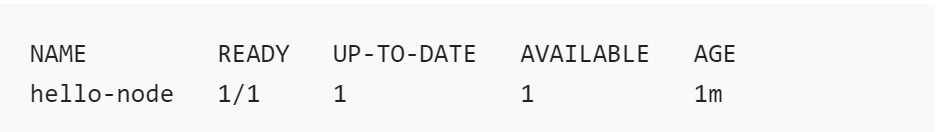
\includegraphics{images/output_get_deployment.png}
        \caption{get deployment}
        \label{fig:deployment}
    \end{figure}
    \item Per visualizzare il POD utilizzare il comando
    \begin{lstlisting}
        kubectl get pods
    \end{lstlisting}
    \begin{figure}[h]
        \centering
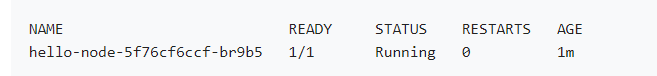
\includegraphics{images/output_pods.png}
        \caption{Output PODS}
        \label{fig:output_pods}
    \end{figure}
    \item Per visualizzare gli eventi del cluster
    \begin{lstlisting}
        kubectl get events
    \end{lstlisting}
      \begin{figure}[h]
        \centering
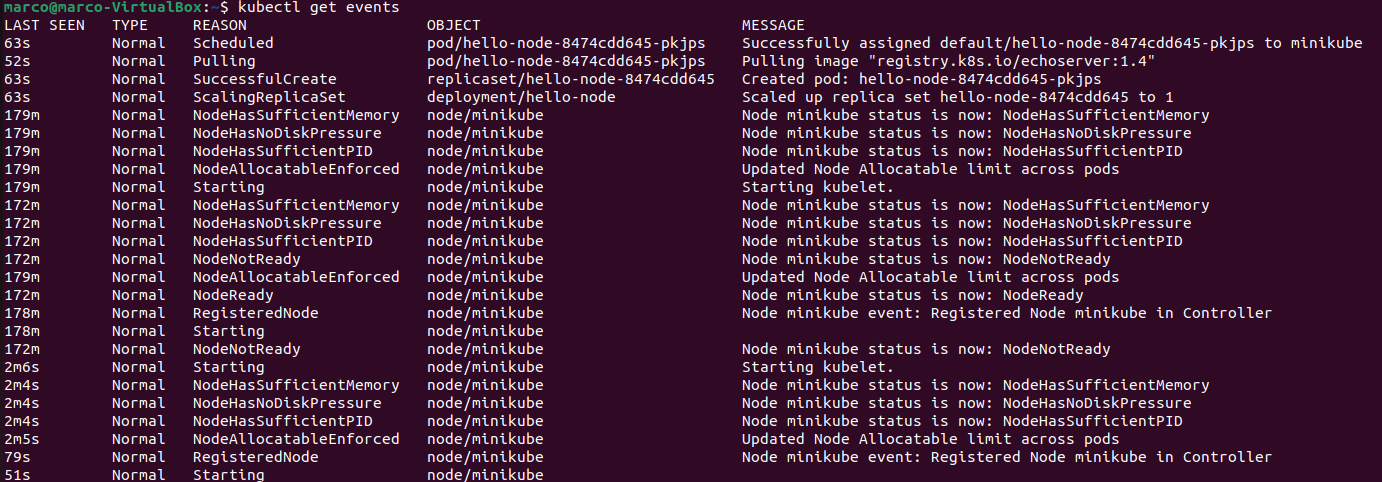
\includegraphics[width=0.7\textwidth]{images/get_events.png}
        \caption{Get events}
        \label{fig:get_events}
    \end{figure}
    \item Per visualizzare le configurazioni kubectl    \begin{lstlisting}
        kubectl config view
    \end{lstlisting}
     \begin{figure}[h]
        \centering
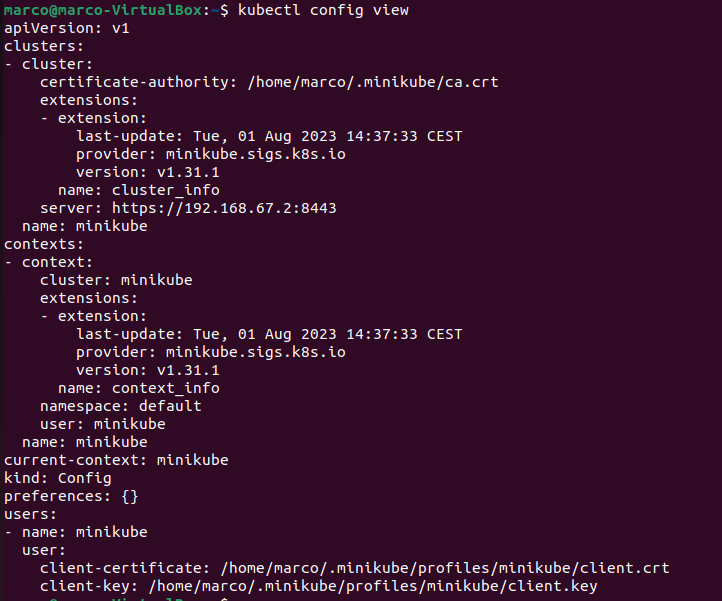
\includegraphics[width=0.7\textwidth]{images/get_config_view.png}
        \caption{Config view}
        \label{fig:config_view}
    \end{figure}
\end{enumerate}

\section{Implementazione}
\subsection{Apache Kafka}
Le note riportate si riferiscono ad un sistema operativo Linux dove è già stata scaricata una versione di \textbf{Apache Kafka}. I comandi devono essere eseguiti dalla cartella di installazione.
\begin{itemize}
    \item mandare in esecuzione il gestore \textbf{Zookeeper}
    \begin{lstlisting}
    bin/zookeeper-server-start.sh config/zookeeper.properties\end{lstlisting}
    \item mandare in esecuzione il \textbf{Broker}
    \begin{lstlisting}
    bin/kafka-server-start.sh config/server.properties\end{lstlisting}
    \item creare un nuovo \textbf{topic} name
   \noindent \begin{lstlisting}
   bin/kafka-topics.sh--create --topic topic--name--bootstrap-serverIP:port server \end{lstlisting}
   \item creare un \textbf{produttore} 
   \begin{lstlisting}
   bin/kafka-console-producer.sh --topic topic--name --bootstrap-server IP:port server \end{lstlisting}
   \item creare un \textbf{consumatore}
   \begin{lstlisting}
   bin/kafka-console-consumer.sh--topic topic--name--from-beginning --bootstrap-server IP:port server
   \end{lstlisting}

\end{itemize}
\pagebreak
\subsection{Creazione di un generatore e consumatore di eventi in python con Apache Kafka}
Come prima operazione di è andati a creare un producer di eventi in python che simuli il cambiamento di stato di un valore.
\begin{lstlisting}[language=Python]
    from time import sleep  
    from json import dumps  
    from kafka import KafkaProducer  
    import random
    import datetime
    import json
    
    producer = KafkaProducer(  
        bootstrap_servers = ['localhost:9092', 'localhost:9093','localhost:9094'],  
        value_serializer = lambda x:json.dumps(x).encode('utf-8')  
        )  
    print("Connect succefully") 
    
    for n in range(50):  
        for j in range(10):
            my_data = {"timestamp": str(datetime.datetime.now()), "id" : str(random.randint(0,999)),"value": random.randint(0,1)} 
            producer.send('druid', value = my_data) 
        print("Send")
        sleep(1) 
    print("End")
\end{lstlisting}
\subsubsection{Svolgimento}
\begin{itemize}
    \item Come prima operazione abbiamo mandato in esecuzione il kluster di nodi \textbf{Apache Kafka} formato da 1 nodo \textbf{Zookeeper} e 3 nodi \textbf{Broker} (Kafka1, Kafka2, Kafka3).
\end{itemize}
\begin{lstlisting}
  networks:
    kafka-druid:
      name: kafka-druid
      driver: bridge
      external: true

services:
  zoo1:
    image: confluentinc/cp-zookeeper:7.3.2
    hostname: zoo1
    networks: 
      - kafka-druid 
    container_name: zoo1
    ports:
      - "2182:2181"
    environment:
      ZOOKEEPER_CLIENT_PORT: 2181
      ZOOKEEPER_SERVER_ID: 1
      ZOOKEEPER_SERVERS: zoo1:2888:3888


  kafka1:
    image: confluentinc/cp-kafka:7.3.2
    hostname: kafka1
    networks: 
      - kafka-druid
    container_name: kafka1
    ports:
      - "9092:9092"
      - "29092:29092"
    environment:
      KAFKA_ADVERTISED_LISTENERS: INTERNAL://kafka1:19092,EXTERNAL://${DOCKER_HOST_IP:-127.0.0.1}:9092,DOCKER://host.docker.internal:29092
      KAFKA_LISTENER_SECURITY_PROTOCOL_MAP: INTERNAL:PLAINTEXT,EXTERNAL:PLAINTEXT,DOCKER:PLAINTEXT
      KAFKA_INTER_BROKER_LISTENER_NAME: INTERNAL
      KAFKA_ZOOKEEPER_CONNECT: "zoo1:2181"
      KAFKA_BROKER_ID: 1
      KAFKA_LOG4J_LOGGERS: "kafka.controller=INFO,kafka.producer.async.DefaultEventHandler=INFO,state.change.logger=INFO"
      KAFKA_AUTHORIZER_CLASS_NAME: kafka.security.authorizer.AclAuthorizer
      KAFKA_ALLOW_EVERYONE_IF_NO_ACL_FOUND: "true"
    depends_on:
      - zoo1

  kafka2:
    image: confluentinc/cp-kafka:7.3.2
    hostname: kafka2
    networks: 
      - kafka-druid
    container_name: kafka2
    ports:
      - "9093:9093"
      - "29093:29093"
    environment:
      KAFKA_ADVERTISED_LISTENERS: INTERNAL://kafka2:19093,EXTERNAL://${DOCKER_HOST_IP:-127.0.0.1}:9093,DOCKER://host.docker.internal:29093
      KAFKA_LISTENER_SECURITY_PROTOCOL_MAP: INTERNAL:PLAINTEXT,EXTERNAL:PLAINTEXT,DOCKER:PLAINTEXT
      KAFKA_INTER_BROKER_LISTENER_NAME: INTERNAL
      KAFKA_ZOOKEEPER_CONNECT: "zoo1:2181"
      KAFKA_BROKER_ID: 2
      KAFKA_LOG4J_LOGGERS: "kafka.controller=INFO,kafka.producer.async.DefaultEventHandler=INFO,state.change.logger=INFO"
      KAFKA_AUTHORIZER_CLASS_NAME: kafka.security.authorizer.AclAuthorizer
      KAFKA_ALLOW_EVERYONE_IF_NO_ACL_FOUND: "true"
    depends_on:
      - zoo1


  kafka3:
    image: confluentinc/cp-kafka:7.3.2
    hostname: kafka3
    networks: 
      - kafka-druid
    container_name: kafka3
    ports:
      - "9094:9094"
      - "29094:29094"
    environment:
      KAFKA_ADVERTISED_LISTENERS: INTERNAL://kafka3:19094,EXTERNAL://${DOCKER_HOST_IP:-127.0.0.1}:9094, DOCKER://host.docker.internal:29094
      KAFKA_LISTENER_SECURITY_PROTOCOL_MAP: INTERNAL:PLAINTEXT,EXTERNAL:PLAINTEXT,DOCKER:PLAINTEXT
      KAFKA_INTER_BROKER_LISTENER_NAME: INTERNAL
      KAFKA_ZOOKEEPER_CONNECT: "zoo1:2181"
      KAFKA_BROKER_ID: 3
      KAFKA_LOG4J_LOGGERS: "kafka.controller=INFO,kafka.producer.async.DefaultEventHandler=INFO,state.change.logger=INFO"
      KAFKA_AUTHORIZER_CLASS_NAME: kafka.security.authorizer.AclAuthorizer
      KAFKA_ALLOW_EVERYONE_IF_NO_ACL_FOUND: "true"
    depends_on:
      - zoo1

\end{lstlisting}
\begin{figure}[h]
    \centering
    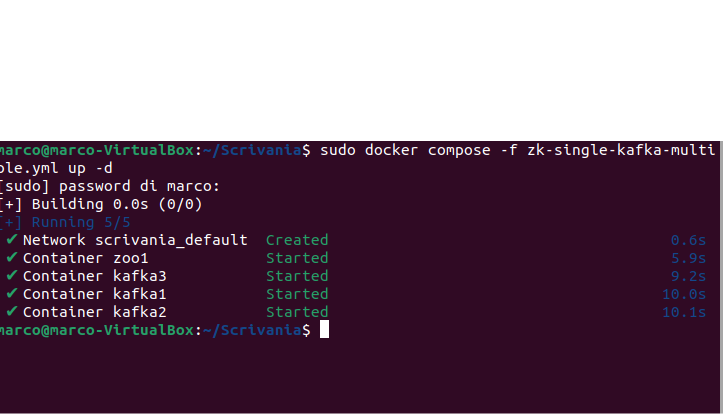
\includegraphics[scale=0.5]{images/kluster_producer.png}
    \caption{Cluster Kafka}
    \label{fig:my_label}
\end{figure}
Dopo di che si è andati a creare un topic in \textbf{Apache Kafka} chiamato \textbf{druid} e si è andati ad eseguire il producer appena creato.
\begin{lstlisting}
  sudo docker exec kafka1 kafka-topics --bootstrap-server kafka1:9092 --create --topic druid
\end{lstlisting}
\pagebreak
\begin{itemize}
    \item Dopo di che siamo andati a creare un consumatore di eventi in python in grado di consumare gli eventi provenienti dal quel topic.
\end{itemize}
\begin{lstlisting}[language=Python]
from json import loads  
from kafka import KafkaConsumer  
import json

consumer = KafkaConsumer(  
    'druid',  
     bootstrap_servers = ['kafka1:9092', 'kafka2:9093','kafka3:9094'],  
     auto_offset_reset = 'earliest',  
     enable_auto_commit = True,  
     group_id = 'my-group',  
     value_deserializer = lambda x : json.loads(x.decode('utf-8'))  
     )  
for message in consumer:  
    message = message.value  
    print(message)      
\end{lstlisting}
\begin{itemize}
  \item Dopo di che per eseguire il producer e il consumatore si è andati ad utilizzare i seguenti comandi su due terminali distinti
\end{itemize}
\begin{lstlisting}
  python3 producer.py
  python3 consumer.py
\end{lstlisting}
\begin{figure}[H]
    \centering
    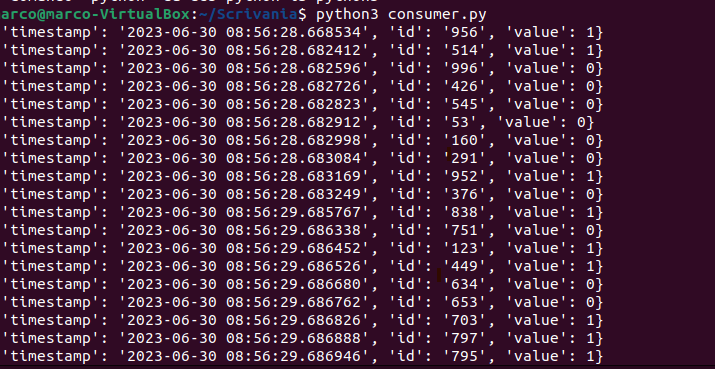
\includegraphics[scale=0.5]{images/consumer.png}
    \caption{Iniezione dei dati}
    \label{fig:my_label}
\end{figure} 
\subsection{Creazione di una data pipeline con Apache Kafka, Apache Druid e Docker Compose}
Le noto riportate in questa sezione illustrano la costruzione e un test di prestazione di una data pipeline containerizzata ed eseguita con \textbf{Docker Compose}.
\subsubsection{Svolgimento}
\begin{itemize}
    \item Come prima operazione si è andati a creare il seguente modello logico relazione, che riporta gli accessi effettuati da degli utenti
    \begin{lstlisting}[language=SQL]
CREATE TABLE accessi(__time TIMESTAMP, nome TEXT, cognome TEXT, indirizzo TEXT, citta TEXT, stato TEXT, cap INT, 
email TEXT, telefono TEXT, eta INT, altezza DECIMAL(5,2), peso DECIMAL(5,2), reddito DECIMAL(6,2), 
datan DATE, professione TEXT, istruzione TEXT, hobby TEXT, nfigli INT, codice_cliente INT, datareg TIMESTAMP);
    \end{lstlisting}
\item Su tale modello dati si è andati a sviluppare il seguente generatore di eventi
\begin{lstlisting}[language=Python]
from time import sleep  
from kafka import KafkaProducer  
import json 
import random
import csv
from faker import Faker
import datetime
producer = KafkaProducer(  
    bootstrap_servers = ["localhost:29092"],  
    value_serializer = lambda x:json.dumps(x).encode("utf-8")  
    )  
print("Connect succefully") 
fake = Faker()
max=random.randint(4,20)
nomi= [fake.first_name() for _ in range(max)]
max=random.randint(4,20)
cognomi= [fake.last_name() for _ in range(max)]
max=random.randint(4,20)
indirizzi= [fake.address() for _ in range(max)]
#la libreria faker genera indirizzi con \n, che vanno sostituiti con uno spazio
for i in range(len(indirizzi)):
    indirizzi[i]=indirizzi[i].replace('\n', ' ')
max=random.randint(4,20)
_citta=[fake.city() for _ in range(max)]
max=random.randint(4,20)
stati=[fake.country() for _ in range(max)]
max=random.randint(4,20)
_cap=[fake.zipcode() for _ in range(max)]
max=random.randint(4,20)
_email=[fake.email() for _ in range(max)]
max=random.randint(4,20)
telefoni=[fake.phone_number() for _ in range(max)]
max=random.randint(4,20)
_eta= [random.randint(18, 89) for _ in range(max)]
max=random.randint(4,20)
altezze= [round(random.uniform(120, 210), 2) for _ in range(max)]
max=random.randint(4,20)
pesi= [round(random.uniform(30, 180), 2) for _ in range(max)]
max=random.randint(4,20)
redditi= [round(random.uniform(1000, 10000), 2) for _ in range(max)]
max=random.randint(4,20)
daten= [fake.date_of_birth(minimum_age=18, maximum_age=89).strftime("%Y-%m-%d") for _ in range(max)]
max=random.randint(4,20)
professioni= [fake.job() for _ in range(max)]
max=random.randint(4,20)
_nfigli= [random.randint(0, 5) for _ in range(max)]
max=random.randint(4,20)
codici_cliente=[fake.random_number(digits=6) for _ in range(max)]
max=random.randint(4,20)
datereg= [fake.date_time_between(start_date="-1y", end_date="now").strftime("%Y-%m-%d %H:%M:%S") for _ in range(max)]
for n in range(500):
    for j in range(10000):
        nome= random.choice(nomi)
        cognome= random.choice(cognomi)
        indirizzo= random.choice(indirizzi)
        citta= random.choice(_citta)
        stato= random.choice(stati)
        cap= random.choice(_cap)
        email= random.choice(_email)
        telefono= random.choice(telefoni)
        eta= random.choice(_eta)
        altezza= random.choice(altezze)
        peso= random.choice(pesi)
        reddito= random.choice(redditi)
        datan= random.choice(daten)
        professione= random.choice(professioni)
        istruzione= fake.random_element(elements=("Scuola Secondaria", "Laurea triennale", "Laurea Magistrale", "Dottorato"))
        hobby= fake.random_element(elements=("Leggere","Viaggiare","Giocare a calcio","Giocare ai videogiochi","Fare sport"))
        nfigli= random.choice(_nfigli)
        codice_cliente= random.choice(codici_cliente)
        datareg= random.choice(datereg)
        accesso= datetime.datetime.now().strftime("%Y-%m-%d %H:%M:%S")
        my_data = {"Accesso": accesso, "nome": nome, "cognome": cognome, "indirizzo": indirizzo, "citta": citta, "stato": stato, "cap": cap,
        "email": email, "telefono": telefono, "eta": eta, "altezza": altezza, "peso": peso,
        "reddito":reddito, "datan":  datan, "professione":  professione, "istruzione": istruzione,
        "hobby": hobby,
        "nfigli": nfigli, "codice_cliente": codice_cliente, 
        "datareg": datareg, 
        }
        producer.send("accessi", value = my_data) 
        sleep(1)

print("End")
     

     

\end{lstlisting}
È possibile notare che è stata applicata una randomici da 4 a 20 sui possibili valori che un attributo può assumere
\item Successivamente è stati creati i servizi di \textbf{Apache Druid} andando a specificare una \textit{docker network} che permetterà ai contaiener di comunicare.
\begin{lstlisting}
version: "2.2"

networks:
  kafka-druid:
    name: kafka-druid
    driver: bridge
    external: true

volumes:
  metadata_data: {}
  middle_var: {}
  historical_var: {}
  broker_var: {}
  coordinator_var: {}
  router_var: {}
  druid_shared: {}


services:
  postgres:
    container_name: postgres
    image: postgres:latest
    networks: 
      - kafka-druid
    ports:
      - "5432:5432"
    volumes:
      - metadata_data:/var/lib/postgresql/data
    environment:
      - POSTGRES_PASSWORD=FoolishPassword
      - POSTGRES_USER=druid
      - POSTGRES_DB=druid
      
  zookeeper:
    container_name: zookeeper
    hostname: zookeeper
    image: confluentinc/cp-zookeeper:7.4.0
    networks: 
      - kafka-druid
    ports:
      - "2181:2181"
    environment:
      - ZOOKEEPER_SERVER_ID=1
      - ZOOKEEPER_CLIENT_PORT=2181

  coordinator:
    image: apache/druid:26.0.0
    container_name: coordinator
    networks:
      - kafka-druid
    volumes:
      - druid_shared:/opt/shared
      - coordinator_var:/opt/druid/var
    depends_on:
      - zookeeper
      - postgres
    ports:
      - "8081:8081"
    command:
      - coordinator
    env_file:
      - environment

  broker:
    image: apache/druid:26.0.0
    container_name: broker
    networks:
      - kafka-druid
    volumes:
      - broker_var:/opt/druid/var
    depends_on:
      - zookeeper
      - postgres
      - coordinator
    ports:
      - "8082:8082"
    command:
      - broker
    env_file:
      - environment

  historical:
    image: apache/druid:26.0.0
    container_name: historical
    networks:
      - kafka-druid
    volumes:
      - druid_shared:/opt/shared
      - historical_var:/opt/druid/var
    depends_on: 
      - zookeeper
      - postgres
      - coordinator
    ports:
      - "8083:8083"
    command:
      - historical
    env_file:
      - environment

  middlemanager:
    image: apache/druid:26.0.0
    container_name: middlemanager
    networks: 
      - kafka-druid
    volumes:
      - druid_shared:/opt/shared
      - middle_var:/opt/druid/var
    depends_on: 
      - zookeeper
      - postgres
      - coordinator
    ports:
      - "8091:8091"
      - "8100-8105:8100-8105"
    command:
      - middleManager
    env_file:
      - environment

  router:
    image: apache/druid:26.0.0
    container_name: router
    networks:
      - kafka-druid
    volumes:
      - router_var:/opt/druid/var
    depends_on:
      - zookeeper
      - postgres
      - coordinator
    ports:
      - "8888:8888"
    command:
      - router
    env_file:
      - environment
\end{lstlisting}
\item  In seguito si è andato a configurare il relativo file di configurazione di \textbf{Apache Druid}
\begin{lstlisting}
#
# Licensed to the Apache Software Foundation (ASF) under one
# or more contributor license agreements.  See the NOTICE file
# distributed with this work for additional information
# regarding copyright ownership.  The ASF licenses this file
# to you under the Apache License, Version 2.0 (the
# "License"); you may not use this file except in compliance
# with the License.  You may obtain a copy of the License at
#
#   http://www.apache.org/licenses/LICENSE-2.0
#
# Unless required by applicable law or agreed to in writing,
# software distributed under the License is distributed on an
# "AS IS" BASIS, WITHOUT WARRANTIES OR CONDITIONS OF ANY
# KIND, either express or implied.  See the License for the
# specific language governing permissions and limitations
# under the License.
#

# Java tuning
#DRUID_XMX=1g
#DRUID_XMS=1g
#DRUID_MAXNEWSIZE=250m
#DRUID_NEWSIZE=250m
DRUID_MAXDIRECTMEMORYSIZE=3072m
DRUID_SINGLE_NODE_CONF=nano-quickstart

druid_emitter_logging_logLevel=debug

druid_extensions_loadList=["druid-histogram", "druid-datasketches", "druid-lookups-cached-global", "postgresql-metadata-storage", "druid-multi-stage-query", "druid-kafka-indexing-service"]

druid_zk_service_host=zookeeper
druid_lookup_enableLookupSyncOnStartup=true
druid_lookup_lookupTierIsDatasource=false
druid_lookup_lookupTier=_default_tier

druid_broker_cache_useCache=true
druid_broker_cache_populateCache=true
druid_broker_cache_useResultLevelCache=true
druid_broker_cache_populateResultLevelCache=true
druid_cache_useCache=true
druid_cache_populateCache=true
druid_cache_useResultLevelCache=true
druid_cache_populateResultLevelCache=true
druid_metadata_storage_host=
druid_metadata_storage_type=postgresql
druid_metadata_storage_connector_connectURI=jdbc:postgresql://postgres:5432/druid
druid_metadata_storage_connector_user=druid
druid_metadata_storage_connector_password=FoolishPassword

druid_coordinator_balancer_strategy=cachingCost

druid_indexer_runner_javaOptsArray=["-server", "-Xmx1g", "-Xms1g", "-XX:MaxDirectMemorySize=3g", "-Duser.timezone=UTC", "-Dfile.encoding=UTF-8", "-Djava.util.logging.manager=org.apache.logging.log4j.jul.LogManager"]
druid_indexer_fork_property_druid_processing_buffer_sizeBytes=256MiB

druid_storage_type=local
druid_storage_storageDirectory=/opt/shared/segments
druid_indexer_logs_type=file
druid_indexer_logs_directory=/opt/shared/indexing-logs

druid_processing_numThreads=1
druid_processing_numMergeBuffers=1

DRUID_LOG4J=<?xml version="1.0" encoding="UTF-8" ?><Configuration status="WARN"><Appenders><Console name="Console" target="SYSTEM_OUT"><PatternLayout pattern="%d{ISO8601} %p [%t] %c - %m%n"/></Console></Appenders><Loggers><Root level="info"><AppenderRef ref="Console"/></Root><Logger name="org.apache.druid.jetty.RequestLog" additivity="false" level="DEBUG"><AppenderRef ref="Console"/></Logger></Loggers></Configuration>

\end{lstlisting}
\item In seguito per mandare in esecuzione i container  
\begin{lstlisting}
    docker compose -f nome_file up -d 
\end{lstlisting}
Dopo tale operazione tutti i container relativi ad \textbf{Apache Druid} saranno in esecuzione
\item Ora si configurano  i container realtvi relativi ad \textbf{Apache Kafka}, per semplicità utilizzeremo un solo nodo come \textbf{Broker} e riutilizzeremo il nodo \textbf{Zookeeper} generato precedentemente come servizio di configurazione dei nodi
\begin{lstlisting}[yaml]
networks:
  kafka-druid:
    name: kafka-druid
    driver: bridge
    external: true

services:
  kafka:
    image: confluentinc/cp-kafka:7.4.0
    hostname: kafka
    container_name: kafka
    networks:
      - kafka-druid
    ports:
      - "29092:29092"
    environment:
      KAFKA_ADVERTISED_LISTENERS: INTERNAL://kafka:9092,EXTERNAL://localhost:29092
      KAFKA_LISTENER_SECURITY_PROTOCOL_MAP: INTERNAL:PLAINTEXT,EXTERNAL:PLAINTEXT
      KAFKA_INTER_BROKER_LISTENER_NAME: INTERNAL
      KAFKA_ZOOKEEPER_CONNECT: "zookeeper:2181"
      KAFKA_BROKER_ID: 1
      KAFKA_LOG4J_LOGGERS: "kafka.controller=INFO,kafka.producer.async.DefaultEventHandler=INFO,
      state.change.logger=INFO"
      KAFKA_OFFSETS_TOPIC_REPLICATION_FACTOR: 1
      KAFKA_TRANSACTION_STATE_LOG_REPLICATION_FACTOR: 1
      KAFKA_TRANSACTION_STATE_LOG_MIN_ISR: 1
      KAFKA_AUTHORIZER_CLASS_NAME: kafka.security.authorizer.AclAuthorizer
      KAFKA_ALLOW_EVERYONE_IF_NO_ACL_FOUND: "true"
\end{lstlisting}
Dopo di che sia il nodo di \textbf{Apache Kafka}, sia quello di \textbf{Apache Druid} saranno in esecuzione. \\
Per lanciare il generatore di eventi lanciare il comando
\begin{lstlisting}
    python3 nome_file.py
\end{lstlisting}
\item in seguito per effettuare l'\textbf{injection} all'interno di \textbf{Apache Druid} usare il servizio gui \textbf{Load data - Streaming-Apache kafka} andando a spedificare  l'hostname e la porta esterna del \textbf{Broker} e il relativi \textbf{topic} di pubblicazione.
\begin{figure}[H]
    \centering
    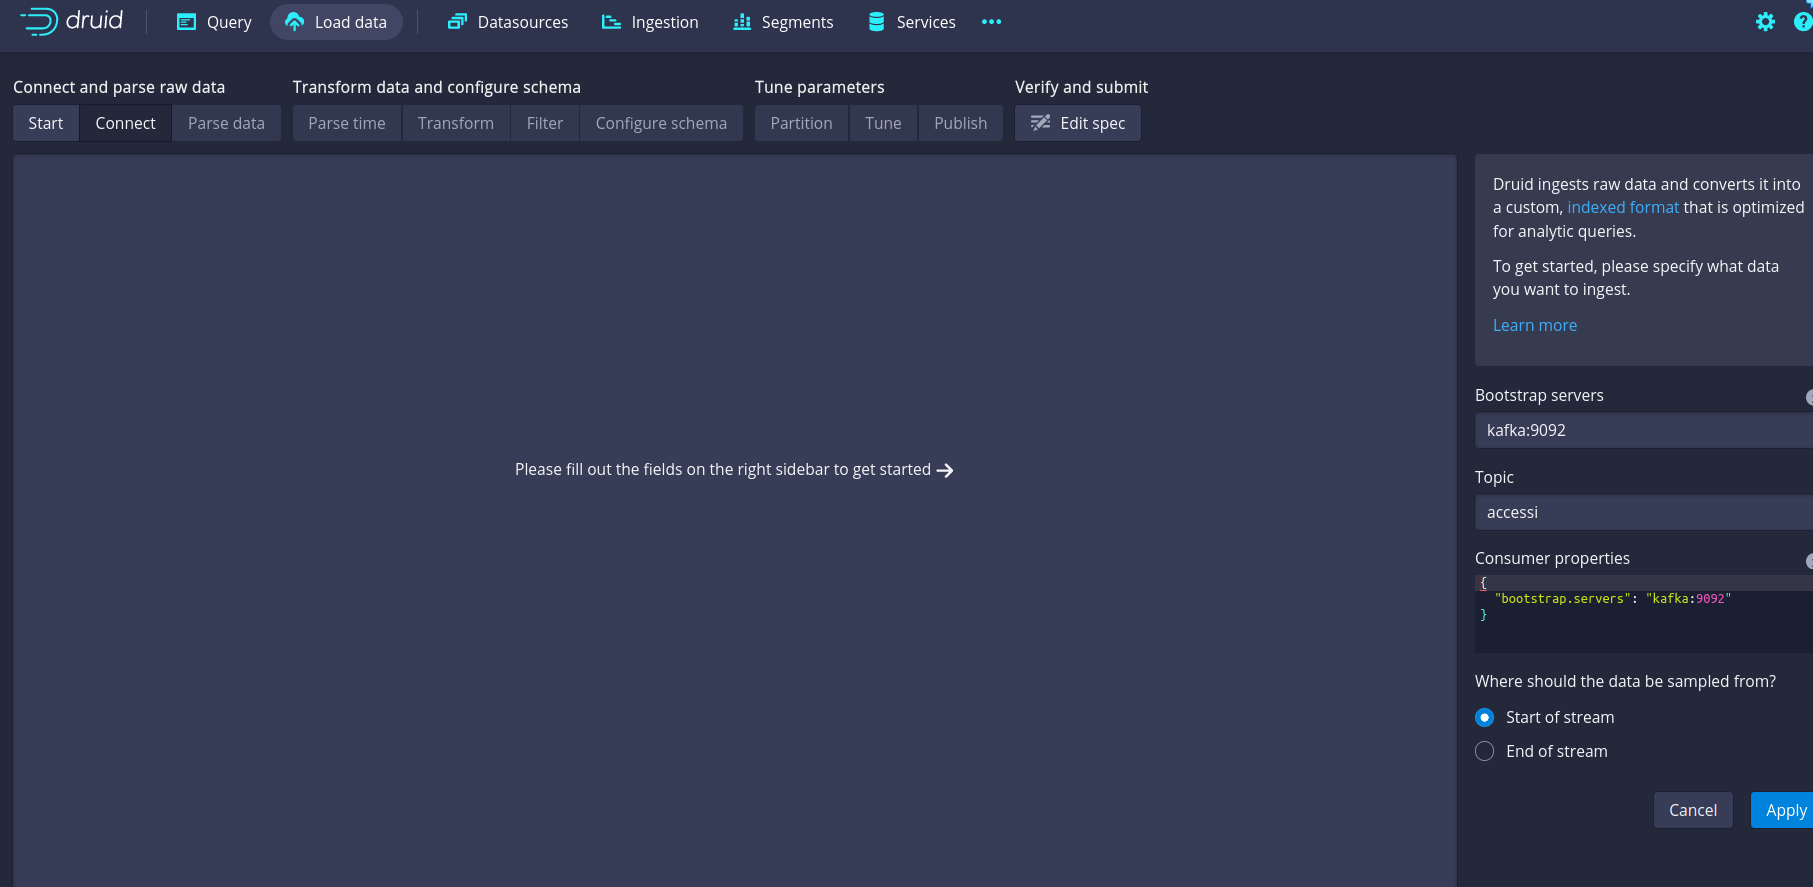
\includegraphics[width=0.8\textwidth]{images/load_data.png}
    \caption{Load data - Streaming-Apache kafka}
\end{figure}
\end{itemize}
\pagebreak
\subsubsection{Confronto tra Apache Druid e Postgres}
Per mettere in evidenza le capacità di questi struemtni andiamo ad utilizzare un datasource da 5000000 record aventi il seguente schema relazione. \\
Per eseguire i comandi direttamente all'interno del container di \textbf{PostgreSQL} eseguire il comando.
\begin{lstlisting}
    sudo docker exec postgres -ti bash 
\end{lstlisting}
\begin{lstlisting}[language=SQL]
CREATE TABLE accessi( nome text, cognome text, indirizzo text, citta text, stato text, cap int, 
email text, telefono text, eta int, altezza decimal(5,2), peso decimal(5,2), reddito decimal(6,2), 
datan date, professione text, istruzione text, hobby text, nfigli int, codice_cliente int, datareg timestamp,__time timestamp);
    
\end{lstlisting}
Utilizzando i seguenti parametri di configurazione per \textbf{Apache Druid} senza l'utilizzo della cache:
\begin{enumerate}
    \item granularity segment per day ;
    \item 800000 max rows in memory.
\end{enumerate}
Inoltre per consentire l'utilizzo degli stessi dati sia in \textbf{Apache Druid} che in \textbf{PostgreSQL},  il generatore degli eventi viene modificato in modo tale da poter memorizzare gli eventi generati all'interno di un file *.csv. 
\pagebreak
\begin{lstlisting}
from time import sleep  
from kafka import KafkaProducer  
import json 
import random
import csv
from faker import Faker
import datetime
producer = KafkaProducer(  
    bootstrap_servers = ["localhost:29092"],  
    value_serializer = lambda x:json.dumps(x).encode("utf-8")  
    )  
print("Connect succefully") 
fake = Faker()
max=random.randint(4,20)
nomi= [fake.first_name() for _ in range(max)]
max=random.randint(4,20)
cognomi= [fake.last_name() for _ in range(max)]
max=random.randint(4,20)
indirizzi= [fake.address() for _ in range(max)]
#la libreria faker genera indirizzi con \n, che vanno sostituiti con uno spazio
for i in range(len(indirizzi)):
    indirizzi[i]=indirizzi[i].replace('\n', ' ')
max=random.randint(4,20)
_citta=[fake.city() for _ in range(max)]
max=random.randint(4,20)
stati=[fake.country() for _ in range(max)]
max=random.randint(4,20)
_cap=[fake.zipcode() for _ in range(max)]
max=random.randint(4,20)
_email=[fake.email() for _ in range(max)]
max=random.randint(4,20)
telefoni=[fake.phone_number() for _ in range(max)]
max=random.randint(4,20)
_eta= [random.randint(18, 89) for _ in range(max)]
max=random.randint(4,20)
altezze= [round(random.uniform(120, 210), 2) for _ in range(max)]
max=random.randint(4,20)
pesi= [round(random.uniform(30, 180), 2) for _ in range(max)]
max=random.randint(4,20)
redditi= [round(random.uniform(1000, 10000), 2) for _ in range(max)]
max=random.randint(4,20)
daten= [fake.date_of_birth(minimum_age=18, maximum_age=89).strftime("%Y-%m-%d") for _ in range(max)]
max=random.randint(4,20)
professioni= [fake.job() for _ in range(max)]
max=random.randint(4,20)
_nfigli= [random.randint(0, 5) for _ in range(max)]
max=random.randint(4,20)
codici_cliente=[fake.random_number(digits=6) for _ in range(max)]
max=random.randint(4,20)
datereg= [fake.date_time_between(start_date="-1y", end_date="now").strftime("%Y-%m-%d %H:%M:%S") for _ in range(max)]
volume=[]
for n in range(500):
    for j in range(10000):
        nome= random.choice(nomi)
        cognome= random.choice(cognomi)
        indirizzo= random.choice(indirizzi)
        citta= random.choice(_citta)
        stato= random.choice(stati)
        cap= random.choice(_cap)
        email= random.choice(_email)
        telefono= random.choice(telefoni)
        eta= random.choice(_eta)
        altezza= random.choice(altezze)
        peso= random.choice(pesi)
        reddito= random.choice(redditi)
        datan= random.choice(daten)
        professione= random.choice(professioni)
        istruzione= fake.random_element(elements=("Scuola Secondaria", "Laurea triennale", "Laurea Magistrale", "Dottorato"))
        hobby= fake.random_element(elements=("Leggere","Viaggiare","Giocare a calcio","Giocare ai videogiochi","Fare sport"))
        nfigli= random.choice(_nfigli)
        codice_cliente= random.choice(codici_cliente)
        datareg= random.choice(datereg)
        accesso= datetime.datetime.now().strftime("%Y-%m-%d %H:%M:%S")
        my_data = {"Accesso": accesso, "nome": nome, "Cognome": cognome, "indirizzo": indirizzo, "citta": citta, "stato": stato, "cap": cap,
        "email": email, "telefono": telefono, "eta": eta, "altezza": altezza, "peso": peso,
        "reddito":reddito, "datan":  datan, "professione":  professione, "istruzione": istruzione,
        "hobby": hobby,
        "nfigli": nfigli, "codice_cliente": codice_cliente, 
        "datareg": datareg, 
        }
        producer.send("accessi", value = my_data) 
        element=[nome, cognome, indirizzo, citta, stato, cap, email, telefono, eta, altezza, peso, reddito, datan, professione, istruzione, hobby, nfigli, codice_cliente, datareg, accesso]
        volume.append(element)
        sleep(1)
with open('data.csv', 'w', newline='') as file:
    writer = csv.writer(file, quoting=csv.QUOTE_NONNUMERIC, delimiter=',')
    writer.writerows(volume) 

print("End")
     

\end{lstlisting}
Per importare i dati contenuti nel file *.csv  all'interno di \textbf{PostgreSQL} utilizzare il seguente comando.
\begin{lstlisting}
COPY accessi(nome, cognome, indirizzo, citta, stato, cap, 
email, telefono, eta, altezza, peso, reddito, 
datan, professione, istruzione, hobby, nfigli, codice_cliente, datareg, __time)
From '/data.csv'
Delimiter ','
csv header;
\end{lstlisting}
\noindent Una volta effettuato l'\textbf{injection} di dati su entrambi i sistemi per misurare le performance si eseguiranno le seguenti query.
\begin{lstlisting}
 - query 1: SELECT DATE_TRUNC('day', __time), citta, COUNT(*)
             FROM accessi
             GROUP BY DATE_TRUNC('day', __time), citta
      
- query 2: SELECT stato, AVG(eta), AVG(reddito)
            FROM accessi
            GROUP BY stato
      
- query 3: SELECT DATE_TRUNC('year', __time), stato, professione, istruzione, nfigli, COUNT(*)
            FROM accessi
            WHERE nfigli> 0
            GROUP BY DATE_TRUNC('year', __time), stato, professione, istruzione, nfigli
            ORDER BY 5 DESC
      
- query 4: SELECT DATE_TRUNC('hour',__time), citta,  AVG(eta)
            FROM accessi
            GROUP BY DATE_TRUNC('hour', __time), citta  

- query 5: SELECT DATE_TRUNC('year', __time), DATE_TRUNC('month', __time), DATE_TRUNC('day', __time), stato, professione, istruzione, nfigli, COUNT(*) 
        FROM accessi
        GROUP BY DATE_TRUNC('year', __time), DATE_TRUNC('month', __time), DATE_TRUNC('day', __time), stato, professione, istruzione, nfigli
        ORDER BY 5 DESC

- query 6: SELECT DATE_TRUNC('year', __time), DATE_TRUNC('month', __time), DATE_TRUNC('day', __time), 
    DATE_TRUNC('hour', __time), stato, professione, istruzione, nfigli, COUNT(*) 
            FROM accessi
            GROUP BY DATE_TRUNC('year', __time), DATE_TRUNC('month', __time), DATE_TRUNC('day', __time), DATE_TRUNC('hour', __time), stato, professione, istruzione, nfigli
            ORDER BY 5 DESC           
\end{lstlisting}
\begin{center}
    \begin{tblr}{
  colspec={XXX},
  row{odd}={bg=lightgray},  
  row{1}={bg=black,fg=white},
}
\centering
 & \centering Apache Druid [s] & \centering PostgreSQL [s] \\\hline 
  \centering
  query1 &  \centering  0.6 & \centering 1.2 \\ \hline
  \centering
  query2 &  \centering 0.2 &  \centering 1.9 \\ \hline 
  \centering
  query3 & \centering 1.2 & \centering 2 \\ \hline
  \centering  query4 & \centering 0.6 & \centering 1.1 \\ \hline
  \centering  query5 & \centering  1.05 & \centering 2.8 \\ \hline
  \centering  query6 & \centering 1.30 & \centering 3.3 \\ \hline
  \end{tblr}
\end{center}
\paragraph{Conclusioni}
Dalla seguente sperimentazione si evince una chiara superiorità di \textbf{Apache Druid} di un ordine di grandezza su un comune database relazione come \textbf{PostgreSQL}, in particolare nell'esecuzione di query che coninvolgono raggrupamenti, anche su intervalli temporali (ora, giorno, mese, anno).
\subsubsection{Confronto tra Apache Druid con e senza rollup}
Per mettere in evidenza la funzionalità di \textbf{rollup} si va a confrontare le prestazioni che \textbf{Apache Druid} sviluppa in un datasource da 5000000 di dati con e senza \textbf{rollup}. Per completezza verrà anche fatto un confronto con un classico database relazione come \textbf{PostgreSQL}.\\
Lo schema relazione è il seguente:
\begin{lstlisting}[language=SQL]
CREATE TABLE accessi(__time timestamp, nome text, cognome text, citta text, stato text, datan date, istruzione text, hobby text); 
\end{lstlisting}
Utilizzando i seguenti parametri per \textbf{Apache Druid} senza l'utilizzo della cache: 
\begin{itemize}
    \item granularity segment per day;
    \item 800000 max rows in memory;
    \item \textbf{roll up} on (per il datasource con \textbf{roll up});
    \item query granularity \textbf{hour}.
\end{itemize}
Per consentire l'utlizzo degli stessi dati anche in \textbf{PostgresSQL} verrà generato un file *.csv contenente tutti i dati generati.\\
Il generatore dei dati è il seguente: 
\begin{lstlisting}[language=Python]
from kafka import KafkaProducer  
import json 
import random
import csv
from faker import Faker
import datetime
producer = KafkaProducer(  
    bootstrap_servers = ["localhost:29092"],  
    value_serializer = lambda x:json.dumps(x).encode("utf-8")  
    )  

print("Connect succefully") 
fake = Faker()
locazione=[[fake.city(), fake.country()] for _ in range(200)]

utenti=list()
for i in range(5000):
    a=locazione[random.randint(0,199)]
    citta=a[0]
    stato=a[1]
    utenti.append([fake.first_name(), fake.last_name(),fake.date_of_birth(minimum_age=18, maximum_age=89).strftime("%Y-%m-%d"), citta, stato, fake.random_element(elements=("Scuola Secondaria", "Laurea triennale", "Laurea Magistrale", "Dottorato")), fake.random_element(elements=("Leggere","Viaggiare","Giocare a calcio","Giocare ai videogiochi","Fare sport")) ] )
volume=[]
for n in range(50):
  
   for j in range(100000):
        accesso=datetime.datetime.now().strftime("%Y-%m-%d %H:%M:%S")
        a=random.randint(0,4999)
        nome=utenti[a][0]
        cognome=utenti[a][1]
        datan=utenti[a][2]
        citta=utenti[a][3]
        stato=utenti[a][4]
        istruzione=utenti[a][5]
        hobby=utenti[a][6]
        my_data = {"accesso": accesso, "nome": nome, "cognome": cognome, "datan":  datan, "citta": citta, "stato": stato, "istruzione": istruzione,
        "hobby": hobby
        }
        producer.send("test_rollup11", value = my_data) 
        element=[nome, cognome, citta, stato, datan,istruzione, hobby,accesso]
        volume.append(element)
with open('data.csv', 'w', newline='') as file:
    writer = csv.writer(file, quoting=csv.QUOTE_NONNUMERIC, delimiter=',')
    writer.writerows(volume) 

print("End")
\end{lstlisting}
Una volta effettuata l'\textbf{injection} dei dati  verrano efettuate le seguenti query per misurare le perfomance richieste.
\begin{lstlisting}
- query 1: SELECT DATE_TRUNC('day', __time), citta, COUNT(*)
            FROM accessi
            GROUP BY DATE_TRUNC('day', __time), citta

            
- query 2: SELECT DATE_TRUNC('year', __time), DATE_TRUNC('month', __time),  stato, COUNT(*)
            FROM accessi
            GROUP BY DATE_TRUNC('year', __time), DATE_TRUNC('month', __time),  stato
            ORDER BY 4 DESC

- query 3: SELECT DATE_TRUNC('year', __time), DATE_TRUNC('month', __time), DATE_TRUNC('day', __time), stato, citta, COUNT(*) 
            FROM accessi
            GROUP BY DATE_TRUNC('year', __time), DATE_TRUNC('month', __time), DATE_TRUNC('day', __time), stato, citta
            ORDER BY 5 DESC


- query 4: SELECT DATE_TRUNC('year', __time), DATE_TRUNC('month', __time), DATE_TRUNC('day', __time), DATE_TRUNC('hour', __time), stato, citta, COUNT(*) 
            FROM accessi
            GROUP BY DATE_TRUNC('year', __time), DATE_TRUNC('month', __time), DATE_TRUNC('day', __time), DATE_TRUNC('hour', __time), stato, citta
            ORDER BY 5 DESC

\end{lstlisting}
\paragraph{Svolgimento}
\begin{itemize}
    \item Per attivare la funzionalità di \textbf{rollup} come prima operazione effettuare lìinjection dei in \textbf{Apache Druid}
    \item In $configure schema$ andare a specificare il campo \textbf{rollup} su \textbf{true} e il campo \textbf{granularity} su \textbf{hour}
    \begin{figure}[H]
        \centering
        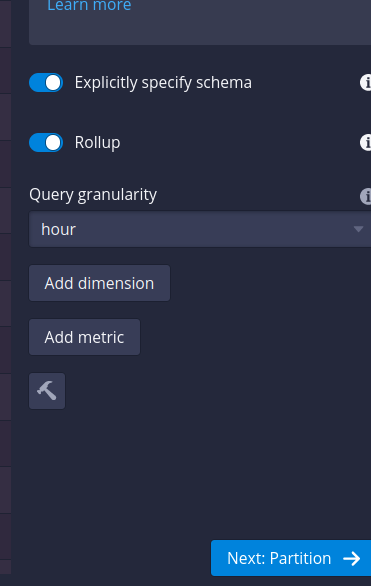
\includegraphics[width=0.3\textwidth]{images/test_rollup.png}
        \caption{Attivazione della funzionalità di rollup}
    \end{figure}
\end{itemize}

\begin{center}
    \begin{tblr}{
  colspec={XXXX},
  row{odd}={bg=lightgray},  
  row{1}={bg=black,fg=white},
}
\centering
 & \centering Apache Druid con rollup[s] & \centering Apache Druid senza rollup [s] & \centering PostgreSQL [s] \\\hline 
  \centering
  query1 &  \centering 0.3  & \centering 0.7 & \centering 0.8 \\ \hline
  \centering query2 &  \centering 0.4 & \centering 0.75 & \centering 1.1 \\ \hline
 \centering
  query3 &  \centering 0.25   & \centering 0.74  & \centering 1.5 \\ \hline
 \centering
  query4 &  \centering 0.16   & \centering 0.8  & \centering 1.6 \\ \hline
  \end{tblr}
\end{center}
\paragraph{Conclusioni}
Come riportato dalla tabella sovrastante, le misure effettuate sul datasource con \textbf{rollup} sono migliori rispetto a quelle effettuate senza \textbf{rollup}, questo perchè grazie a tale funzionalità si riduce il numero di record da processare Seppur la cardinalità dei dati non sia così considerevole, le prestazioni mostrano già una diminuzione di un decimo dal punto di vista delle prestazioni di esecuzione (si passa da 5000000 a 150000 record).
\subsubsection{Utilizzo delle tabelle di lookup in Apache Druid}
Le note riportarte in questa sezione si riferiscono alla creazione e utilizzo delle tabelle di \textbf{lookup} in un classico scenario di \textbf{data enrichment}.
Il modello relazione dei dati generati sarà il seguente: 
\begin{lstlisting}
CREATE TABLE accessi(__time timestamp, citta text, stato text, codice_cliente);
\end{lstlisting}
La tebella di verrà utilizzata per andare a sotituire al \textit{codice\_cliente} il \textit{nome} e il \textit{cognome} del cliente.\\
Il generatore degli eventi è il seguente:
\begin{lstlisting}[language=Python]
  from kafka import KafkaProducer  
  import json 
  import random
  import csv
  from faker import Faker
  import datetime
  producer = KafkaProducer(  
      bootstrap_servers = ["localhost:29092"],  
      value_serializer = lambda x:json.dumps(x).encode("utf-8")  
      )  
  print("Connect succefully") 
  fake = Faker()
  locazione=[[fake.city(), fake.country()] for _ in range(200)]
  
  utenti=list()
  for i in range(150):
      a=locazione[random.randint(0,99)]
      citta=a[0]
      stato=a[1]
      a=random.randint(0,999)
      utenti.append([a, fake.first_name(), fake.last_name(),fake.date_of_birth(minimum_age=18, maximum_age=89).strftime("%Y-%m-%d"), citta, stato] )
  
  for i in range(150):
   print('\"'+str(utenti[i][0])+"\""+":"+"\""+utenti[i][1]+" "+utenti[i][2]+"\"")
  volume=[]
  for n in range(500):
      accesso=datetime.datetime.now().strftime("%Y-%m-%d %H:%M:%S")
      codice=utenti[random.randint(0,149)][0]
      nome=utenti[random.randint(0,149)][1]
      cognome=utenti[random.randint(0,149)][2]
      datan=utenti[random.randint(0,149)][3]
      citta=utenti[random.randint(0,149)][4]
      stato=utenti[random.randint(0,149)][5]
      my_data = {"accesso": accesso, "codice_cliente": str(codice),  "datan":  datan, "citta": citta, "stato": stato,
      }
      producer.send("lookup", value = my_data) 
      element=[codice, nome, cognome, citta, stato, datan, accesso]
      volume.append(element)
  with open('data.csv', 'w', newline='') as file:
      writer = csv.writer(file, quoting=csv.QUOTE_NONNUMERIC, delimiter=',')
      writer.writerows(volume) 
  print("End")
\end{lstlisting}
Una volta effettuata l'\textbf{injection} dei dati, si va a creare la tabella di \textbf{lookup} chiamata $tabella1$.
\begin{figure}[H]
    \centering
    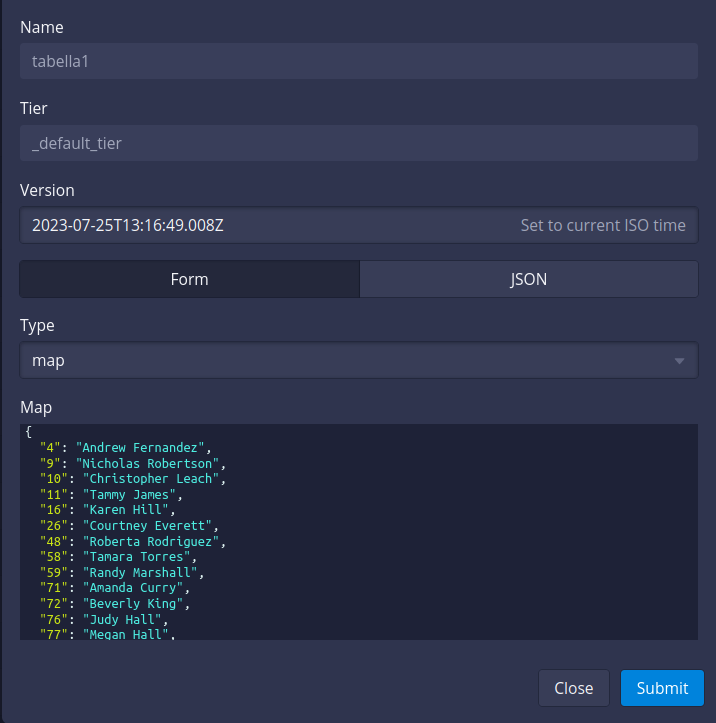
\includegraphics[width=0.5\textwidth]{images/inserimento_lookup.png}
    \caption{Creazione della tabella di lookup}
\end{figure}
In seguito si è andati ad eseguire la seguente query per verificare il corretto funzionamento della tabella di \textbf{lookup}.
\begin{lstlisting}
  SELECT LOOKUP(codice_cliente,'tabella1'), datan, citta, stato
  FROM accessi
\end{lstlisting}
\begin{figure}[H]
    \centering
    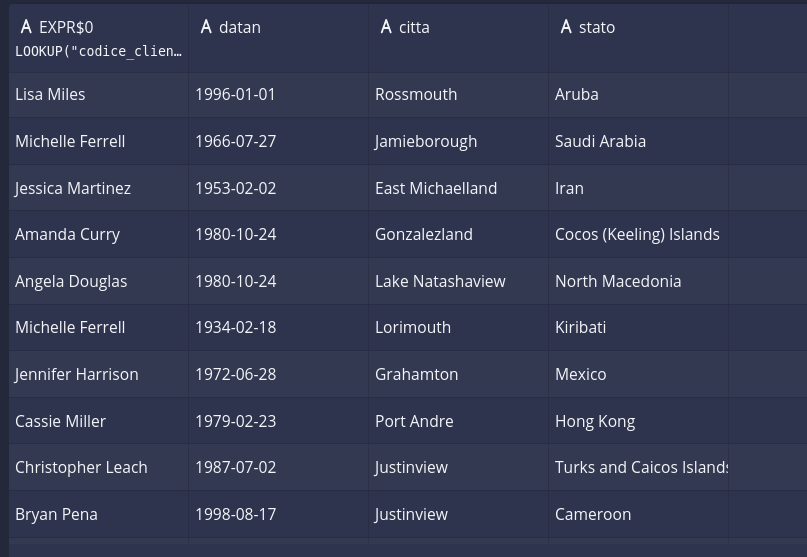
\includegraphics[width=0.5\textwidth]{images/lookup.png}
    \caption{Risultato della query utilizzando la tabella di lookup}
\end{figure}
\section{Test}
\subsection{High Availability}
Per andare a testare l'alta affidabilità, si è andati a creare un cluster di nodi formato da: 1 nodo Zookeeper, 3 nodi broker (Kafka1, Kafka2, Kafka3) e si è andati ad istanziare un produttore e consumatore collegati al broker Kafka1. Ora per testare l'alta affidabilità basta simulare un malfunzionamento e verificare se i messaggi che il broker Kafka1 non è riuscito ad inviare al consumatore sono accessibili attraverso i server Kafka2 e Kafka3. 

\subsubsection{Svolgimento}
\begin{itemize}
    \item Come prima operazione si è andati a creare un cluster di 3 nodi Kafka e un nodo ZooKeeper utilizzando Docker Compose, utilizzando il comando
    \begin{lstlisting}
        sudo docker compose -f nome_file_Kafka.yml up -d 
    \end{lstlisting}
\end{itemize}

\begin{figure}[H]
    \centering
    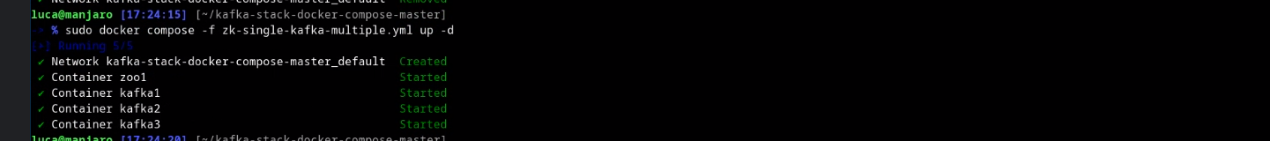
\includegraphics[scale=0.5]{images/cluster.png}
    \caption{Creazione del cluster}
    \label{fig:my_label}
\end{figure}
\begin{itemize}
    \item Creazione del topic "test".
\end{itemize}
\begin{lstlisting}
    sudo docker exec kafka1 kafka-topics --bootstrap-server kafka1:19092 --create --topic topic_name
\end{lstlisting}
\begin{figure}[H]
    \centering
    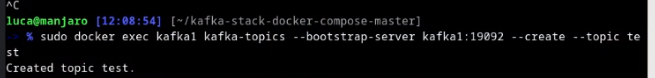
\includegraphics[scale=0.5]{images/create_topic.png}
    \caption{Creazione del topic}
    \label{fig:my_label}
\end{figure}
\begin{itemize}
    \item Creazione di produttore e consumatore.
\end{itemize}
\begin{lstlisting}
    sudo docker exec --interactive --tty kafka1 kafka-console-producer --bootstrap-server kafka1:19092 kafka2:19093 kafka3:19094 --topic topic_name 
\end{lstlisting}
\begin{figure}[H]
    \centering
    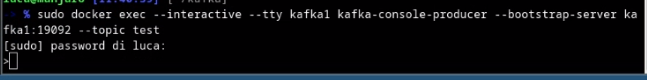
\includegraphics[scale=0.5]{images/produttore.png}
    \caption{Creazione del produttore}
    \label{fig:my_label}
\end{figure}
\begin{lstlisting}
    sudo docker exec --interactive --tty kafka1 kafka-console-consumer --bootstrap-server kafka1:19092 kafka2:19093 kafka3:19094 --topic topic_name --from-beginning
\end{lstlisting}
\begin{figure}[H]
    \centering
    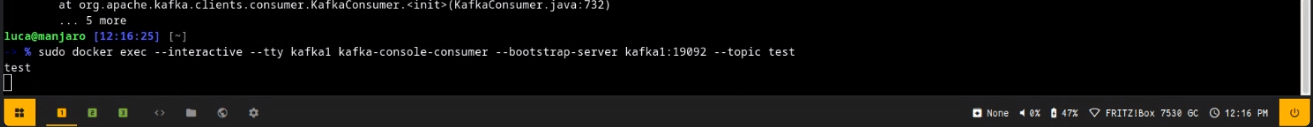
\includegraphics[scale=0.5]{images/consumatore.png}
    \caption{Creazione del consumatore}
    \label{fig:my_label}
\end{figure}
\begin{itemize}
    \item Se il nodo kafka1 viene spento, il produttore e consumatore possono continuare a comunicare collegandosi o al nodo kafka2 o al nodo kafka3.
\end{itemize}
\begin{figure}[H]
    \centering
    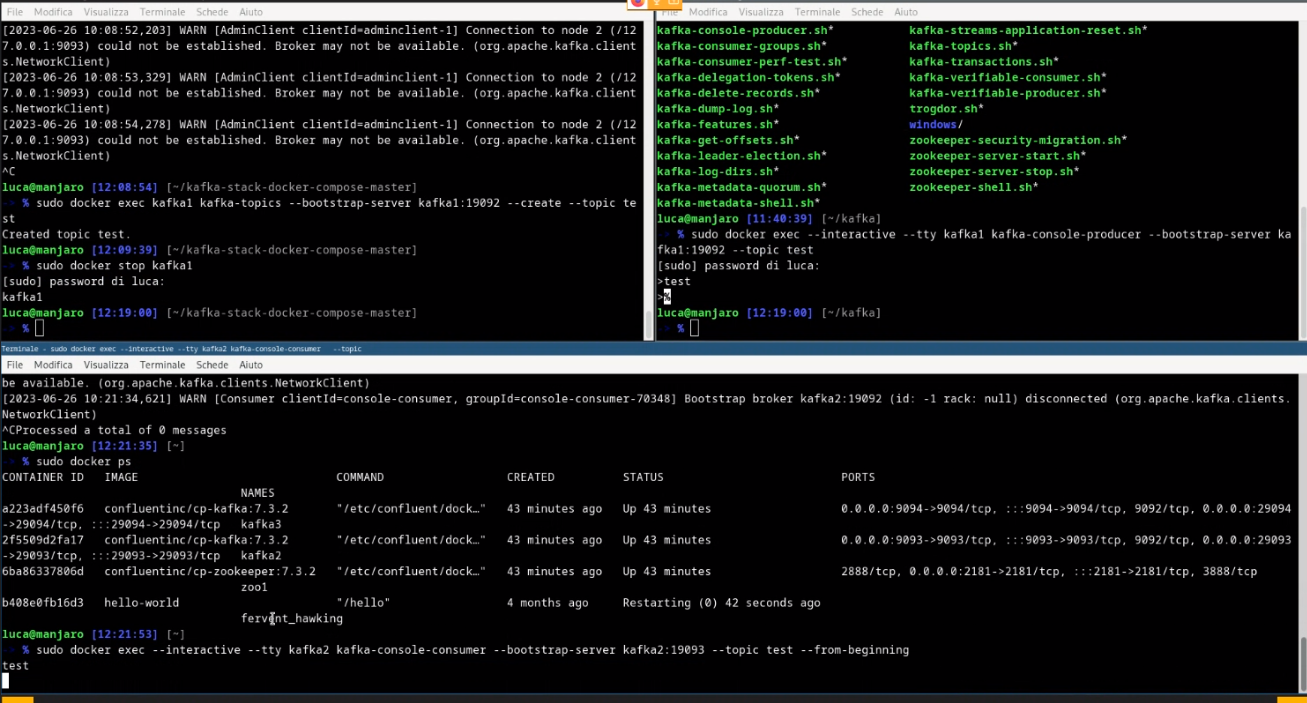
\includegraphics[scale=0.5]{images/test_di_high_avaibility.png}
    \caption{Test di alta affidabilità}
    \label{fig:my_label}
\end{figure}
\subsection{Verifica di connessione al container da un altro host}
Per andare a verificare la connessione al container a partire da un altro host non facciamo altro che conneterci al container attraverso la porta pubblica che espone, configurata nel parametro external di configurazione.
\subsubsection{Svolgimento}
\begin{itemize}
    \item Come prima operazione si è andati a creare un cluster di 3 nodi Kafka e un nodo ZooKeeper utilizzando Docker Compose.
\end{itemize}
\begin{figure}[H]
    \centering
    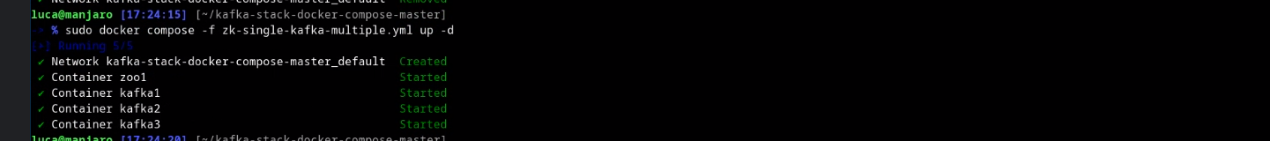
\includegraphics[scale=0.5]{images/cluster.png}
    \caption{Creazione del cluster}
    \label{fig:my_label}
\end{figure}
\begin{itemize}
    \item Dopo di che abbiamo creato dei topic da esempio.
\end{itemize}
\begin{figure}[H]
    \centering
    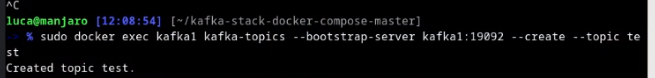
\includegraphics[scale=0.5]{images/create_topic.png}
    \caption{Creazione dei topic}
    \label{fig:my_label}
\end{figure}
\begin{itemize}
    \item Ed infine ci siamo collegati al cluster a partire da un altro host (localhost) per visualizzare la lista dei topic creati.
\end{itemize}
\begin{lstlisting}
   bin/kafka-topics.sh --list --bootstrap-server localhost:9093
\end{lstlisting}
\begin{figure}[H]
    \centering
    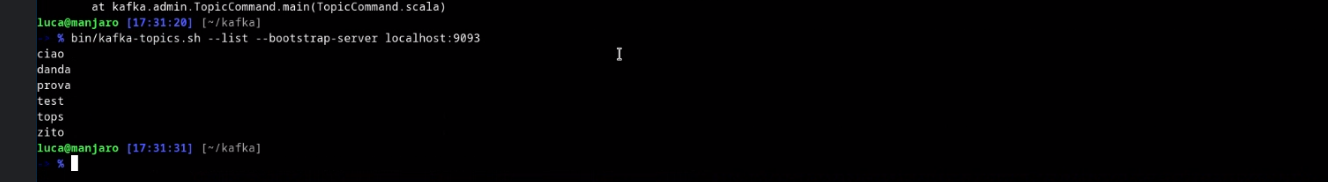
\includegraphics[scale=0.5]{images/test_connect_another_host.png}
    \caption{Connessione da altro host}
    \label{fig:my_label}
\end{figure}
\bibliographystyle{IEEEtran}
\bibliography{https://Kafka.apache.org/documentation/}
\bibliography{https://ably.com/topic/pub-sub#the-pub-sub-model-explained}
\bibliography{https://kafka.apache.org/quickstart}
\bibliography{https://druid.apache.org/docs/latest/ingestion/rollup.html}
\bibliography{https://kubernetes.io/docs/concepts/overview/}
\bibliography{https://kubernetes.io/docs/tutorials/hello-minikube/}
\bibliography{https://www.redhat.com/sysadmin/kubeconfig}
\end{document}
